\documentclass[9pt,a4paper]{report}

\PassOptionsToPackage{table}{xcolor}
\usepackage[table]{xcolor}
\usepackage{geometry}
\usepackage{titlesec}
\usepackage{fancyhdr}
\usepackage{tikz}
\usetikzlibrary{patterns,calc}
\usepackage{tcolorbox}
\tcbuselibrary{skins,breakable,listings}
\usepackage{booktabs}
\usepackage{array}
\usepackage{todonotes}
\usepackage{longtable}
\usepackage{enumitem}
\usepackage{listings}
\usepackage{caption}
\usepackage{tabularx}
\newcolumntype{Y}{>{\centering\arraybackslash}X}
\usepackage{multicol}
\usepackage{multirow}
\usepackage[hidelinks]{hyperref}
\usepackage{bookmark}
\usepackage{lastpage}
\usepackage{float}
\usepackage{amsmath, amsthm, amsfonts}
\usepackage{xstring}
\usepackage{times}
\renewcommand{\familydefault}{\sfdefault}
\usepackage[scaled=1]{inconsolata} 

\usepackage[color]{register}
\usetikzlibrary{positioning,arrows.meta,fit,backgrounds}

\makeatletter
% Draw only the value row (no bit-number row)
\newcommand{\regfieldvalue}[5][]{%
  \setRegLengths%
  \setlength{\regFieldLen}{#3\regFieldLen+\fboxrule}%
  \setcounter{lowerbit}{#4}%
  \setcounter{upperbit}{#4+#3-1}%
  \ifx\relax#1\relax%
    % No color
    \makebox[0pt][l]{%
      \raisebox{-\regResetDrop}{%
        \framebox[\regFieldLen][c]{%
          \regResetSize%
          \rule[-\regResetDepth]{0pt}{\regResetHeight}%
          \regSpread{#5}}}}%
  \else
    % Colored box
    \makebox[0pt][l]{%
      \raisebox{-\regRsvdDrop}{%
        \setlength\fboxsep{0pt}%
        \colorbox{#1}{%
          \framebox[\regFieldLen][c]{%
            \regResetSize%
            \rule[-\regResetDepth]{0pt}{\regRsvdHeight}%
            \raisebox{\regFboxSep}{%
              \makebox[\regFieldLen]{%
                \hspace{\regFboxSep}\regSpread{#5}\hspace{\regFboxSep}}}}}%
        \setlength\fboxsep{\regFboxSep}}}%
  \fi
  \makebox[\regFieldLen]{}%
  \hspace{-\fboxrule}%
}
\makeatother

\geometry{a4paper,left=25mm,right=22mm,top=25mm,bottom=25mm,headheight=12pt}

\definecolor{docNavy}{RGB}{0,42,79}
\definecolor{docBlue}{RGB}{0,118,206}
\definecolor{docLightBlue}{RGB}{223,238,247}
\definecolor{docGray}{RGB}{89,89,89}
\definecolor{docPaleGray}{RGB}{244,245,246}
\definecolor{docLine}{RGB}{204,209,214}
\definecolor{docWarnRed}{RGB}{178,32,38}
\definecolor{docNoteGreen}{RGB}{31,122,90}

% Remove extra space above/below items and keep lists compact
\setlist{
  itemsep=2pt,       % Space between successive items
  parsep=0pt,        % Space between paragraphs WITHIN a single item
  topsep=4pt,        % Space above and below the entire list
  partopsep=0pt      % Extra space added if list starts a new paragraph
}

\titleformat{\chapter}[block]
  {\normalfont}
  {}
  {0pt}
  {\chapterbar}
\titlespacing*{\chapter}{0pt}{0pt}{10mm}

\newcommand{\chapterbar}{
  \colorbox{docNavy}{
    \parbox[c][15mm]{\textwidth}{\hspace{4mm}%
      \textcolor{white}{\fontsize{11}{13}\selectfont\bfseries CHAPTER \thechapter}}%
  }\\[5mm]
  \Large\bfseries\color{docNavy}
}

\titleformat{name=\chapter,numberless}[block]
  {\normalfont}
  {}
  {0pt}
  {\Large\bfseries\color{docNavy}}
\titlespacing*{name=\chapter,numberless}{0pt}{10mm}{10mm}

\titleformat{\section}
  {\Large\bfseries\color{docNavy}}{\thesection}{3mm}{}%
\titleformat{\subsection}
  {\large\bfseries\color{docNavy}}{\thesubsection}{3mm}{}%
\titleformat{\subsubsection}
  {\normalsize\bfseries\color{docGray}}{\thesubsubsection}{3mm}{}%

\titlespacing*{\section}{0pt}{7mm}{4mm}
\titlespacing*{\subsection}{0pt}{5mm}{3mm}
\titlespacing*{\subsubsection}{0pt}{4mm}{2mm}

\pagestyle{fancy}
\fancyhf{}
\renewcommand{\headrulewidth}{0.6pt}
\renewcommand{\footrulewidth}{0.4pt}
\renewcommand{\headrule}{{\color{docLine}\hrule width\headwidth height\headrulewidth}}
\renewcommand{\footrule}{{\color{docLine}\hrule width\headwidth height\footrulewidth}}

\newcommand{\docShortTitle}{Technical Reference Manual}
\newcommand{\docCode}{DOC-0001-EN}

\fancyhead[LE]{\small\color{docGray}\docShortTitle}
\fancyhead[RO]{\small\color{docGray}\leftmark}
\fancyfoot[LE,RO]{\small\color{docGray}\docCode}
\fancyfoot[CE,CO]{\small\color{docGray}\thepage\ of \pageref{LastPage}}
\fancyfoot[RE,LO]{\small\color{docBlue}\bfseries Libre-V (v1.0)}

\fancypagestyle{plain}{%
  \fancyhf{}
  \renewcommand{\headrulewidth}{0pt}
  \fancyfoot[CE,CO]{\small\color{docGray}\thepage\ of \pageref{LastPage}}
  \fancyfoot[RE,LO]{\small\color{docBlue}\bfseries Libre-V (v1.0)}
  \fancyfoot[LE,RO]{\small\color{docGray}\docCode}
}

\lstdefinestyle{docCode}{
  backgroundcolor=\color{docPaleGray},
  basicstyle=\ttfamily\small,
  keywordstyle=\color{docNavy}\bfseries,
  commentstyle=\color{docGray}\itshape,
  stringstyle=\color{docBlue},
  numbers=left,
  numberstyle=\tiny\color{docGray},
  numbersep=6pt,
  frame=single,
  rulecolor=\color{docLine},
  framesep=6pt,
  xleftmargin=2pt,
  breaklines=true,
  showstringspaces=false,
  tabsize=2,
}
\lstset{style=docCode}
\renewcommand{\lstlistingname}{Example}

\newtcolorbox{docnote}{
  breakable, enhanced, colback=docLightBlue, colframe=docBlue,
  boxrule=0pt, leftrule=3pt, arc=0pt, outer arc=0pt,
  left=8pt, right=8pt, top=5pt, bottom=5pt,
  fonttitle=\bfseries\color{docBlue},
  title={NOTE}
}
\newtcolorbox{doccaution}{
  breakable, enhanced, colback=docPaleGray, colframe=docGray,
  boxrule=0pt, leftrule=3pt, arc=0pt, outer arc=0pt,
  left=8pt, right=8pt, top=5pt, bottom=5pt,
  fonttitle=\bfseries\color{docGray},
  title={CAUTION}
}
\newtcolorbox{docwarning}{
  breakable, enhanced, colback=red!5, colframe=docWarnRed,
  boxrule=0pt, leftrule=3pt, arc=0pt, outer arc=0pt,
  left=8pt, right=8pt, top=5pt, bottom=5pt,
  fonttitle=\bfseries\color{docWarnRed},
  title={WARNING}
}

% Code box: a tcolorbox wrapping listings, sharing the docCode style.
% Optional argument takes tcb keys plus a convenience `lang` key:
%   \begin{doccode}                        ... \end{doccode}
%   \begin{doccode}[lang=C]                ... \end{doccode}
%   \begin{doccode}[lang=C,title={boot.c}] ... \end{doccode}
\tcbset{lang/.style={listing options={style=docCode, frame=none, backgroundcolor=, numbers=none, xleftmargin=0pt, language=#1}}}
\newtcblisting{doccode}[1][]{
  breakable, enhanced,
  colback=docPaleGray, colframe=docLine,
  boxrule=0.6pt, arc=0pt, outer arc=0pt,
  left=6pt, right=6pt, top=4pt, bottom=4pt,
  fonttitle=\ttfamily\bfseries\small\color{docNavy},
  coltitle=docNavy, colbacktitle=docLightBlue,
  listing only,
  listing options={style=docCode, frame=none, backgroundcolor=, numbers=none, xleftmargin=0pt},
  #1
}

\newcommand{\makeCoverPage}[5]{%
  \begin{titlepage}
  \newgeometry{left=0mm,right=0mm,top=0mm,bottom=0mm}
  \begin{tikzpicture}[remember picture,overlay]
    \fill[docNavy] (current page.south west) rectangle (current page.north east);
    \begin{scope}
      \clip (current page.north east) rectangle ++(-9,-9);
      \foreach \i in {0,...,14}{
        \draw[docBlue,opacity=0.35,line width=0.8pt]
          ($(current page.north east)+(-9+\i*0.65,0)$) -- ++(9,-9);
      }
    \end{scope}
    % bright accent block bottom-left
    \fill[docBlue] (current page.south west) rectangle ++(4.2,4.2);
    \fill[white,opacity=0.12] (current page.south west) rectangle ++(4.2,4.2);
    % thin accent rule under the logo lockup
    \node[anchor=north west] at ($(current page.north west)+(2.2,-2.2)$) {%
      \begin{tikzpicture}
        \node[anchor=north west] at ($(current page.north west)+(2.2,-2.2)$) {%
        \begin{tikzpicture}
            \node[anchor=west] at (1.75,0.21) {
\includegraphics[width=4.5cm]{figures/logo_colored.pdf}};
        \end{tikzpicture}%
        };
      \end{tikzpicture}%
    };

    % Title block
    \node[anchor=north west,text width=15.5cm,align=left] at ($(current page.north west)+(2.2,-9.5)$)
      {\color{white}\fontsize{34}{40}\selectfont\bfseries #1\par};
    \node[anchor=north west,text width=15cm,align=left] at ($(current page.north west)+(2.2,-13.8)$)
      {\color{docBlue!55!white}\fontsize{16}{20}\selectfont #2\par};
    % accent rule
    \draw[docBlue,line width=1.6pt] ($(current page.north west)+(2.2,-14.9)$) -- ++(6,0);
    % Meta info block bottom
    \node[anchor=south west,text width=15.5cm,align=left] at ($(current page.south west)+(2.2,4.9)$)
      {\color{white}\small
       \begin{tabular}{@{}ll@{}}
        %  \textbf{Document number:} & #3 \\[2pt]
         \textbf{Version:}         & #4 \\[2pt]
         \textbf{Date:}            & #5 \\[2pt]
         \textbf{Status:}          & Under Development
       \end{tabular}%
      };
  \end{tikzpicture}
  \restoregeometry
  \end{titlepage}
}

\setlength{\parindent}{0pt}
\setlength{\parskip}{6pt}
\linespread{1.05}

\hypersetup{
  colorlinks=true,
  linkcolor=docBlue,
  citecolor=docNavy,
  urlcolor=docBlue,
  pdftitle={\docShortTitle},
}

\newcommand{\regtitle}[2]{
  \subsection*{Register #1: #2}
}

\newcommand{\regmeta}[5]{
  \begin{tabular}{@{}ll@{}}
    \toprule
    \textbf{Property} & \textbf{Value} \\
    \midrule
    Base address      & #1 \\
    Byte offset       & #2 \\
    Reset value       & #3 \\
    Access type       & #4 \\
    Bus data width    & 32-bit (only bits [7:0] are used) \\
    Register width    & 8 bits \\
    \bottomrule
  \end{tabular}\\[0.5em]
  \textit{#5}
}

\newenvironment{regmap}{
  \begin{longtable}{@{}p{1.6cm}p{2.4cm}p{1.2cm}p{1.4cm}p{7.8cm}@{}}
    \toprule
    \textbf{Bit(s)} & \textbf{Name} & \textbf{Type} & \textbf{Reset} & \textbf{Description} \\
    \midrule
    \endhead
}{
    \bottomrule
  \end{longtable}
}

\begin{document}

\renewcommand{\docShortTitle}{Technical Reference Manual}
\renewcommand{\docCode}{Stanford University}
\newcommand{\aytooc}{I\textsuperscript{2}C}

\makeCoverPage
  {Libre-V (v1.0)\\ {\LARGE An Open-Source RISC-V SoC.}}
  {User Reference}
  {Stanford University}
  {1.0}
  {\today}

\pagenumbering{roman}
\chapter*{About this Document}
\addcontentsline{toc}{chapter}{About this Document}

This document serves as the reference manual for the Libre-V System-on-Chip (SoC). It describes the SoC's functional blocks, their configuration options, and their intended usage. The manual is intended for software developers and hardware designers working with Libre-V platform at any abstraction.

\subsection*{Release information}
\addcontentsline{toc}{section}{Release Information}
\begin{tabularx}{\textwidth}{@{}l l X@{}}
\toprule
\textbf{Version} & \textbf{Date} & \textbf{Changes} \\
\midrule
1.0 & Aug 2026 & Initial release. \\
\bottomrule
\end{tabularx}

\subsection*{Conventions used in this manual}
\addcontentsline{toc}{section}{Conventions}
\begin{itemize}[leftmargin=*]
  \item \textbf{Monospace} text indicates register names, field names, signal names, or code.
  \item \textit{Italic} text indicates a value that you must supply.
  \item Bit ranges are written \texttt{[hi:lo]}, for example \texttt{[7:4]}.
  \item \colorbox{docLightBlue}{\textcolor{docBlue}{\textbf{Blue}}} panels highlight notes; \colorbox{red!5}{\textcolor{docWarnRed}{\textbf{red}}} panels highlight warnings and cautions the user should be careful about.
\end{itemize}

\subsection*{Abbreviations}
\addcontentsline{toc}{section}{Abbreviations}
\begin{tabular}{c l}
  RF & Register File \\
  RO & Read-Only Access \\
  RW & Read-Write Access \\
  WO & Write-Only Access (Reads are undefined/ have no meaning)\\
\end{tabular}

\subsection*{Notes}
\addcontentsline{toc}{section}{Notes}
\begin{itemize}
  \item The official ARM/AMBA specifications have replaced the master--slave terminology with manager--subordinate. However, some parts of the Libre-V were developed before this terminology change and the legacy master--slave nomenclature may appear in corresponding source code.
  \item The base implementation/specification refers to the SoC configuration that you get on cloning the repository. It is possible to configure the SoC to your needs using a Terminal User Interface. Note that this feature is still in beta testing stage and is not recommended for use without caution. 
\end{itemize}


\tableofcontents
\listoffigures
\listoftables

\clearpage
\pagenumbering{arabic}

\part{Architecture and Software View}

This part is intended for audience intending to understand the platform's architecture, configure, and adopt it in their own system. 

\chapter{Architecture}
\begin{figure}[htbp]
    \centering
    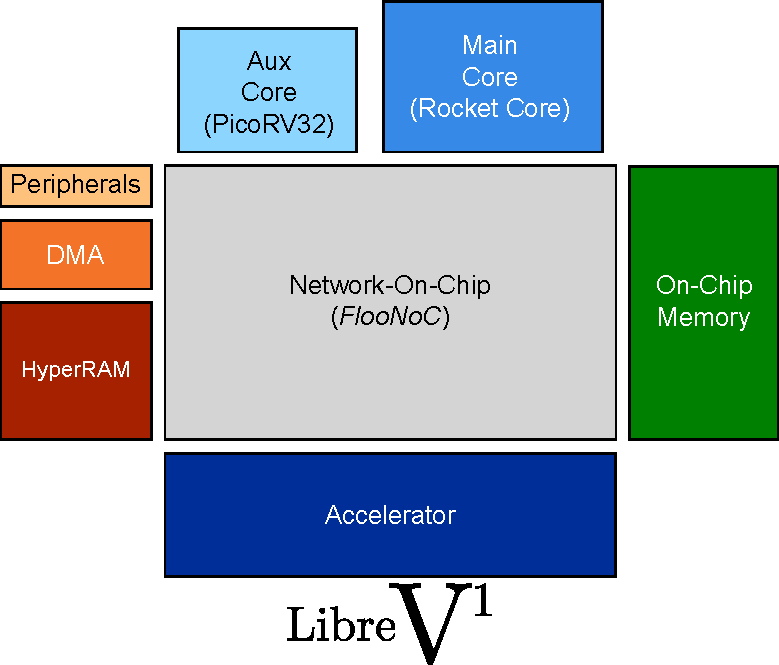
\includegraphics[width=0.65\textwidth]{figures/libre_concept.pdf}
    \caption{Libre-V system-on-chip concept.}
    \label{fig:soc-concept}
\end{figure}

\section{Overview}
Libre-V is a configurable system-on-chip platform intended to be used as host-CPU for testing ASICs, especially accelerators. Being composed of all open-source components, it is completely open source and licensed under the Apache-2.0 license\footnote{Individual components may be protected by their own licensing. Refer the \href{https://code.stanford.edu/tambe-lab/base-soc-v2/-/blob/main/README.md}{repository} for more details.}. The platform uses a 32-bit auxilary core coupled with a 64-bit main core. The auxilary core implements RV32IMC instruction set, whereas the main core implements RV64GC instruction set.  

\begin{docwarning}
    This is document does not discuss the implementation of either the RISC-V ISA nor any of the individual SoC components. For that, we direct the reader to the documentation available at \href{https://riscv.org/specifications/ratified/}{respective source(s)}.  
\end{docwarning}

\section{System}

\begin{figure}[htbp]
  \centering
  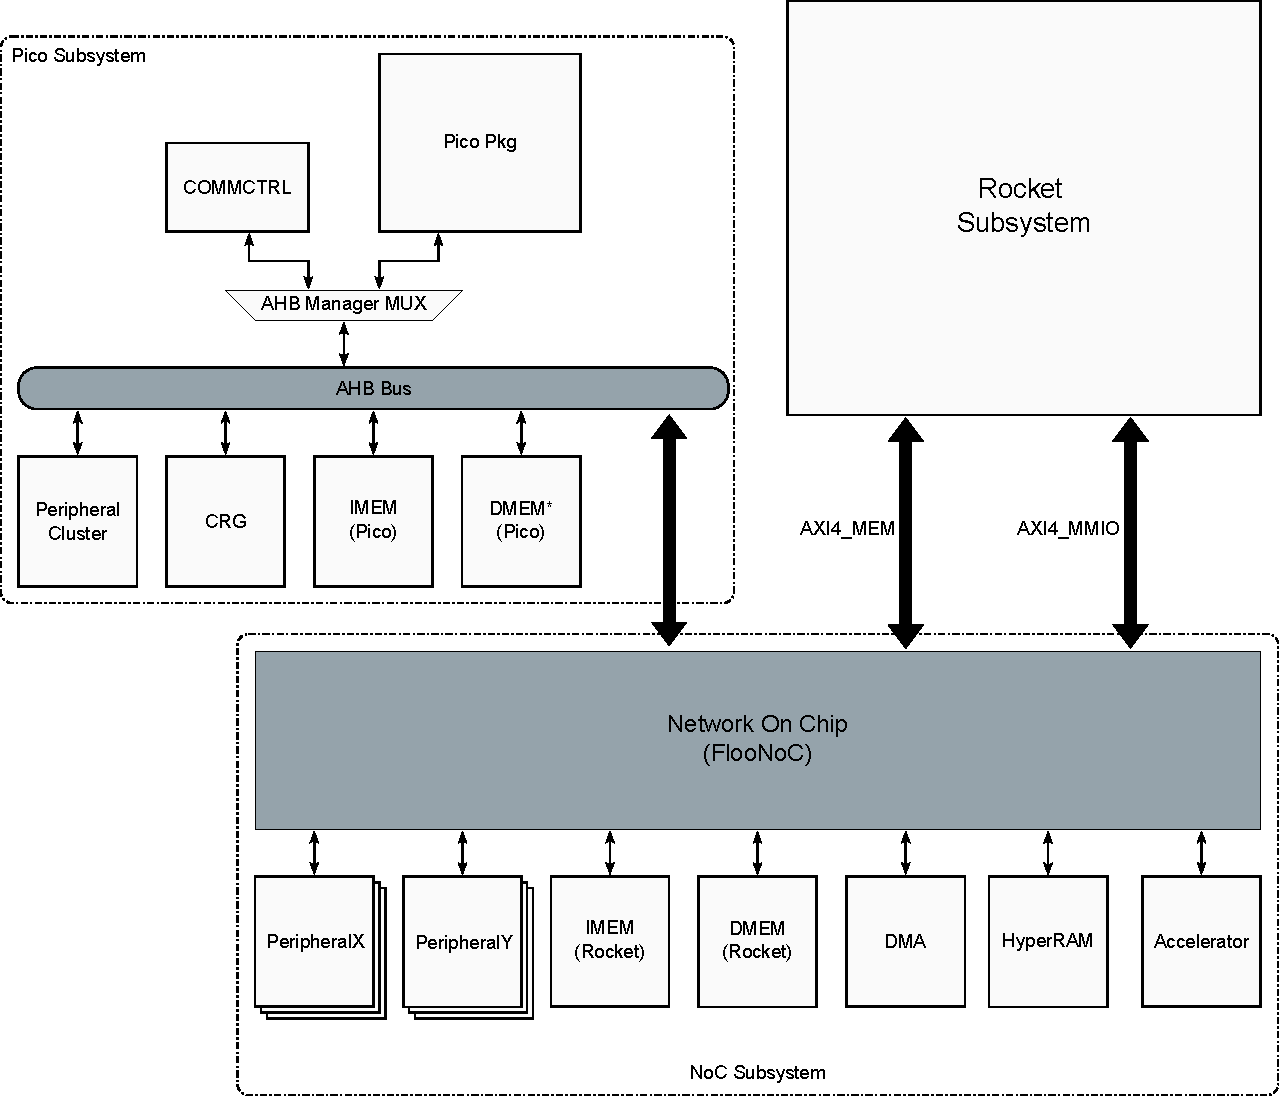
\includegraphics[width=0.95\textwidth]{figures/libre_top_blk.pdf}
  \caption{Libre-V platform block view.}
  \label{fig:top-blk}
\end{figure}

Libre-V platform has 32-bit address space shared by memory-mapped I/O devices. It is composed of three subsystems: 

\begin{enumerate}
    \item Pico Subsystem
    \item Rocket Subsystem 
    \item Network on Chip (NoC) Subsystem
\end{enumerate}

See Figure~\ref{fig:top-blk} for a block-view of the platform. Note that the figure only shows two peripheral groups in the NoC subsystem. However, this is only meant for illustrations. It is possible to configure an Libre-V instance with more than 2 peripherals.

This part of the manual provides a software view of each  component of the Libre-V:  
\begin{itemize}
    \item \hyperref[ch:sw-pico-sys]{Pico Subsystem}
    \item \hyperref[ch:sw-rocket-sys]{Rocket Subsystem}
    \item \hyperref[ch:sw-uart]{UART}
    \item \hyperref[ch:sw-timer]{Timer}
    \item \hyperref[ch:compiling-firmware]{Libre Firmware and Device Drivers}
    \item \hyperref[ch:libre-boot]{Libre Booting Process}     
\end{itemize}
% TODO: Fix all the forward links and add the new entries. 

\newpage

\chapter{Pico Subsystem}\label{ch:sw-pico-sys}

\begin{figure}[htbp]
    \centering
    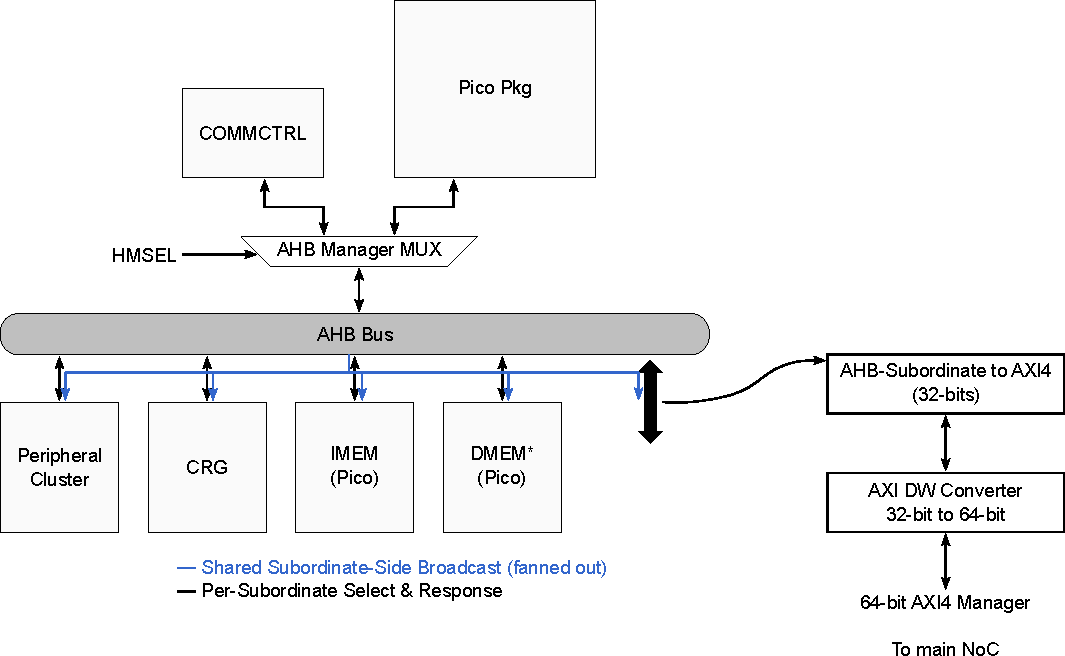
\includegraphics[width=0.95\textwidth]{figures/pico_subsys_blk.pdf}
    \caption{Pico subsystem block view.}
    \label{fig:picosys-blk}
\end{figure}

The Pico subsystem is the SoC's control plane. It couples the PicoRV32 core (as \hyperref[sec:sw-pico-pkg]{Pico Package}) with the host command interface, \hyperref[sec:sw-commctrl]{COMMCTRL}, the on-chip control registers (\hyperref[sec:sw-crg]{CRG}), and the Pico-local peripherals (\hyperref[sec:sw-peripheral-cluster]{Peripheral Cluster}), all joined by an \hyperref[sec:sw-ahb-bus]{AHB Bus}. It is the first block to wake at power-on and is responsible for loading and releasing the Rocket core (\autoref{ch:sw-rocket-sys}). See Figure~\ref{fig:picosys-blk}. 

\section{Pico Package}\label{sec:sw-pico-pkg}

PicoRV32 core is a lightweight, auxilary core developed by Yosys. It implements RV32IMC instruction set. More generally, it can be configured as an RV32E, RV32I, RV32IC, RV32IM, RV32IMC core. It has the following features\footnote{PPA results reproduced here from the repository without any additional verification.}:
\begin{itemize}
  \item Small, lightweight core requiring about 750 -- 2000 LUTs in 7-Series Xilinx Architecture. 
  \item High \(f_\mathrm{max}\) of about 250 -- 450 MHz on Xilinx FPGAs. 
  \item Three options for interfaces: Native Memory (\texttt{picorv32}), AXI4-Lite Manager (\texttt{picorv32\_axi}), or Wishbone (\texttt{picorv32\_wb}).
  \item A built-in interrupt controller with optional, custom ISA support.
  \item An optional co-processor interface. 
  \item Configurable RF: It is possible to disable support for the registers \texttt{x16 - x32}, as well as \texttt{RDCYCLE[H]}, \texttt{RDTIME[H]}, and \texttt{RDINSTRET[H]} instructions\footnote{Refer to the official RV32E ISA.}. The RF can be configured as single or dual ported. 
\end{itemize}

\textbf{Relevant Link(s):} \begin{itemize}
  \item \href{https://github.com/YosysHQ/picorv32}{PicoRV32 Repository}
  \item \href{https://github.com/whatmough/CHIPKIT.git}{COMMCTRL/CHIPKIT Repository}
  \item \href{https://github.com/adki/gen_amba_2021.git}{AMBA Bus Generator Repository}
\end{itemize}

The \texttt{pico\_pkg\_ahb} bridges the native-memory PicoRV32 core to the subsystem as a single AHB-Lite manager. The package attaches the core's private on-chip SRAM memory and fixes the boot
convention:
\begin{center}
  \begin{tabular}{c c}
    \toprule
    \textbf{Region} & \textbf{Base} \\
    \midrule
    .global, .text, .rodata, .data & \texttt{0x0000.0000}\\
    Stack & \\
    \bottomrule
  \end{tabular}
\end{center}

The reset vector is \texttt{0x0000.0000}, and the initial stack pointer\todo{FIX THIS RATIO!} is placed at the top of the print-buffer region (\texttt{0x0001.FC00}). The host loads Pico firmware into IMEM through COMMCTRL before handover.

\section{COMMCTRL}\label{sec:sw-commctrl}

The COMMCTRL is a UART-based communication controller. It is capable of accessing i.e., reading and writing to any address in the 32-bit address space\footnote{The address should have meaning of course, else it might cause an illegal access trap somewhere in the SoC or return a garbage value.}. To use this module, UART interface is exposed over which binary form of the ASCII representation of the read and/or write commands is stream. 

The format of a write command is as follows:
\begin{center}
    \begin{tabular}{c c}
        \toprule 
        Byte & Field \\
        \midrule
        0 & ASCII (W or w)\\
        1 & single whitespace \\
        2 & 0 \\
        3 & ASCII(X or x)\\
        4 - 11 & WRADDR \\
        12 & single whitespace \\
        13 & 0 \\
        14 & ASCII(X/x) \\
        15 - 22 & WRDATA \\
        23 & CR \\
        24 & LF \\
        \bottomrule
    \end{tabular}
\end{center}
and a read command is formatted as:
\begin{center}
    \begin{tabular}{c c}
        \toprule 
        Byte & Field \\
        \midrule
        0 & ASCII (R or r)\\
        1 & single whitespace \\
        2 & 0 \\
        3 & ASCII(X or x)\\
        4 - 11 & RDADDR \\
        12 & CR \\
        13 & LF \\
        \bottomrule
    \end{tabular}
\end{center}
While the write command is 25 bytes large, the read command is shorter and is zero-padded to match this length. As shown in Figure~\ref{fig:picosys-blk}, the COMMCTRL and Pico package are multiplexed as managers of the AHB-Lite bus. The control of this AHB MUX is handled by writing to the location 0x1000.0000. Particularly, writing a 1 to this location using the COMMCTRL hands over the control to the Pico package. Writing a 0 relinquishes the control back to the COMMCTRL. 

Because it is a bus master, the host can load the Pico IMEM, load the Rocket memories across the NoC, and
read results back. 
\begin{center}
  \begin{tabular}{@{}lll@{}}
  \toprule
  \textbf{Address} & \textbf{Symbol} & \textbf{Effect} \\
  \midrule
  \texttt{0x1000\_0000} & \texttt{COMMCTRL\_HANDOVER\_ADDR} & Host writes 1 to hand bus ownership to the Pico. \\
  \texttt{0x1000\_0004} & \texttt{COMMCTRL\_IRQ\_ADDR}      & Host write raises a one-cycle COMMCTRL interrupt. \\
  \bottomrule
  \end{tabular}
\end{center}


\section{AHB Manager MUX and Bus}\label{sec:sw-ahb-bus}
The \texttt{pico\_ahb\_bus} is the subsystem interconnect. It arbitrates two managers, COMMCTRL and the Pico core, onto one AHB fabric and decodes the address to select a subordinate. Ownership is
explicit: at power-on COMMCTRL holds the bus and loads memory; when the host writes the handover address (\autoref{sec:sw-commctrl}), ownership passes to the Pico core, which then runs its firmware. Addresses that do not fall in a local subordinate are forwarded to the NoC through the AHB-to-AXI bridge (\autoref{ch:hw-pico-sys}). 

The address space \texttt{0x0000.0000 - 0x2000.0000} is reserved for the managers of the PicoSys and includes the on-chip SRAM memory of the Pico core, the control registers defined by CRG, and the peripheral cluster.   

\section{Clock and Reset Generator (CRG)}\label{sec:sw-crg}

\section{Peripheral Cluster}\label{sec:sw-peripheral-cluster}
% \chapter{Rocket Subsystem}\label{ch:sw-rocket-sys}

\section{Overview}
The main core of Libre-V is a 64-bit Rocket core, generated from the Chips Alliance
\texttt{rocket-chip} generator. It is a single ``big'' in-order core implementing RV64GC, with private
L1 instruction and data caches and a broadcast coherence hub (there is no L2). Virtual memory is
disabled in the base configuration (\texttt{WithoutVM}); the core runs in bare physical addressing, and
the I\$/D\$ TLBs perform only PMP/PMA permission and cacheability checks.

\begin{docwarning}
This document does not describe the Rocket microarchitecture or the RISC-V ISA. For those, consult the
\href{https://github.com/chipsalliance/rocket-chip}{rocket-chip} documentation and the ratified RISC-V
specifications.
\end{docwarning}

The Rocket connects to the rest of the SoC through \textbf{two} AXI4 master ports, split by
cacheability, so the core never caches side-effecting device registers:
\begin{itemize}[nosep]
  \item \textbf{\texttt{mem\_axi4}} (cacheable) --- behind the coherence hub. Carries L1 refills and
        writebacks to real memory. Covers \texttt{0x8000\_0000}--\texttt{0xFFFF\_FFFF}
        (Rocket instruction/data SRAMs, HyperRAM).
  \item \textbf{\texttt{mmio\_axi4}} (uncacheable) --- hangs directly off the system bus and bypasses
        the coherence hub, so its region advertises no cacheable access and device reads/writes are
        never cached. Covers \texttt{0x1000\_0000}--\texttt{0x7FFF\_FFFF} (UART1, TIMER1, DMA,
        accelerator).
\end{itemize}
Both windows start at or above \texttt{0x1000\_0000}; the low 256\,MiB stays private to the Rocket
(Debug, BootROM, CLINT, PLIC).

\section{Rocket-Private Devices}
These devices are internal to the tile and never leave it. Their addresses are the rocket-chip defaults.

\begin{longtable}{@{}llll@{}}
\toprule
\textbf{Device} & \textbf{Base} & \textbf{Range} & \textbf{Notes} \\
\midrule
\endhead
Debug Module & \texttt{0x0000\_0000} & 4\,KB & DMI/JTAG debug; tied off in Libre-V. \\
Error device & \texttt{0x0000\_3000} & 4\,KB & Catches bad accesses. \\
Boot ROM     & \texttt{0x0001\_0000} & 64\,KB & Reset vector (\texttt{\_hang}) at \texttt{0x0001\_0040}. \\
CLINT        & \texttt{0x0200\_0000} & 64\,KB & \texttt{msip}@+0x0, \texttt{mtimecmp}@+0x4000, \texttt{mtime}@+0xBFF8. \\
PLIC         & \texttt{0x0C00\_0000} & 64\,MB & priority@+0x0, pending@+0x1000, enables@+0x2000, threshold/claim@+0x20\_0000. \\
\bottomrule
\end{longtable}

\section{Memory Map Seen by the Rocket}
Beyond the private devices, everything the Rocket reaches leaves on one of the two master ports and is
routed by the NoC. The instruction/data placement below is a software convention, not a hardware split:
the Rocket has a unified physical map fed by the I\$ (fetch) and D\$ (load/store) through the cacheable
port, and has no on-tile RAM.

\begin{tabular}{@{}llll@{}}
\toprule
\textbf{Use} & \textbf{Base} & \textbf{Port} & \textbf{NoC endpoint} \\
\midrule
Program image  & \texttt{0x8000\_0000} & \texttt{mem\_axi4}  & \texttt{sram\_imem\_rocket} (256\,KB) \\
Data           & \texttt{0x8010\_0000} & \texttt{mem\_axi4}  & \texttt{sram\_dmem\_rocket} (256\,KB) \\
HyperRAM       & \texttt{0xA000\_0000} & \texttt{mem\_axi4}  & \texttt{hyperram} \\
UART1          & \texttt{0x2000\_0000} & \texttt{mmio\_axi4} & \texttt{uart1} \\
TIMER1         & \texttt{0x2010\_0000} & \texttt{mmio\_axi4} & \texttt{timer1} \\
DMA            & \texttt{0x2020\_0000} & \texttt{mmio\_axi4} & \texttt{dma\_sub} \\
Accelerator    & \texttt{0x3000\_0000} & \texttt{mmio\_axi4} & \texttt{accelerator} \\
\bottomrule
\end{tabular}

\section{Interrupts (PLIC)}
The Rocket takes external interrupts through its PLIC. Libre-V wires five external lines, one
independent source per device (nothing is OR'd together):

\begin{tabular}{@{}cll@{}}
\toprule
\textbf{PLIC source} & \textbf{Symbol} & \textbf{Device} \\
\midrule
1 & \texttt{ROCKET\_PLIC\_SRC\_DMA}      & DMA completion \\
2 & \texttt{ROCKET\_PLIC\_SRC\_ACCEL}    & Accelerator (\autoref{ch:sw-accel}) \\
3 & \texttt{ROCKET\_PLIC\_SRC\_TIMER1\_A}& TIMER1 overflow \\
4 & \texttt{ROCKET\_PLIC\_SRC\_TIMER1\_B}& TIMER1 compare match \\
5 & \texttt{ROCKET\_PLIC\_SRC\_UART1}    & UART1 \\
\bottomrule
\end{tabular}

Software uses the PLIC in the usual way: set a per-source priority, raise the enable bit, lower the
context threshold, then claim/complete inside the trap handler. Machine timer and software interrupts
come from the CLINT (\texttt{mtimecmp}/\texttt{msip}). The Pico core drives \emph{no} Rocket interrupt
line; the two cores communicate through shared memory and the boot handshake below.

\section{Boot Mechanism}\label{sec:rocket-boot}
The Rocket has no DMI/JTAG boot path in the base configuration. It is started by the Pico over the CRG:

\begin{enumerate}[nosep]
  \item At power-on the Rocket is held in reset by the CRG gate \texttt{DC\_ROCKET\_RSTN}, which resets
        to \texttt{0}. The Pico subsystem shares the start-up clock and wakes first.
  \item The Pico (or the host through COMMCTRL, \autoref{ch:sw-pico-sys}) loads the Rocket program into
        \texttt{sram\_imem\_rocket} at \texttt{0x8000\_0000} and its data, then writes a boot sentinel
        (\texttt{0xB007C0DE}) to the last word of the instruction region (\texttt{0x8003\_FFFC}). Because
        the load path is in-order, the sentinel's arrival proves every image write has landed.
  \item The Pico polls that sentinel, then releases the Rocket by writing \texttt{DC\_ROCKET\_RSTN = 1}.
  \item Reset release is the trigger: the hart runs the BootROM reset vector (\texttt{\_hang} at
        \texttt{0x0001\_0040}), which clears the chicken bits and jumps to \texttt{DRAM\_BASE}
        (\texttt{0x8000\_0000}). There is no PLIC setup or \texttt{wfi} wait in the reset path.
\end{enumerate}

\begin{docnote}
Because the D\$ is write-back, data the Rocket produces (for example a result buffer another master will
read) stays dirty in the cache until it is flushed. Flush the affected range before signalling
completion to another master.
\end{docnote}

\section{Source Files}

\begin{tabular}{@{}ll@{}}
\toprule
\textbf{File} & \textbf{Role} \\
\midrule
\texttt{rocket\_subsystem/rocket\_subsystem.sv} & Hand-written wrapper: packs the flat AXI ports onto the NoC structs \\
\texttt{rocket\_subsystem/rocket\_generated/} & Generated Rocket RTL (from \texttt{LibreRocketConfig}) \\
\texttt{rocket\_subsystem/generator/\ldots/LibreRocketConfig.scala} & Configuration (ports, VM, coherence hub) \\
\texttt{rocket\_subsystem/generator/bootrom/libre\_bootrom.S} & Custom BootROM (reset-release-and-go) \\
\texttt{software/libre\_rocket.h} & Firmware view: addresses, PLIC sources, cache helpers \\
\bottomrule
\end{tabular}

\newpage

\chapter{Universal Asynchronous Receiver/Transmitter (UART)}\label{ch:sw-uart}

\section{Overview}\label{sec:uart-constr}
\begin{figure}[htbp]
  \centering
  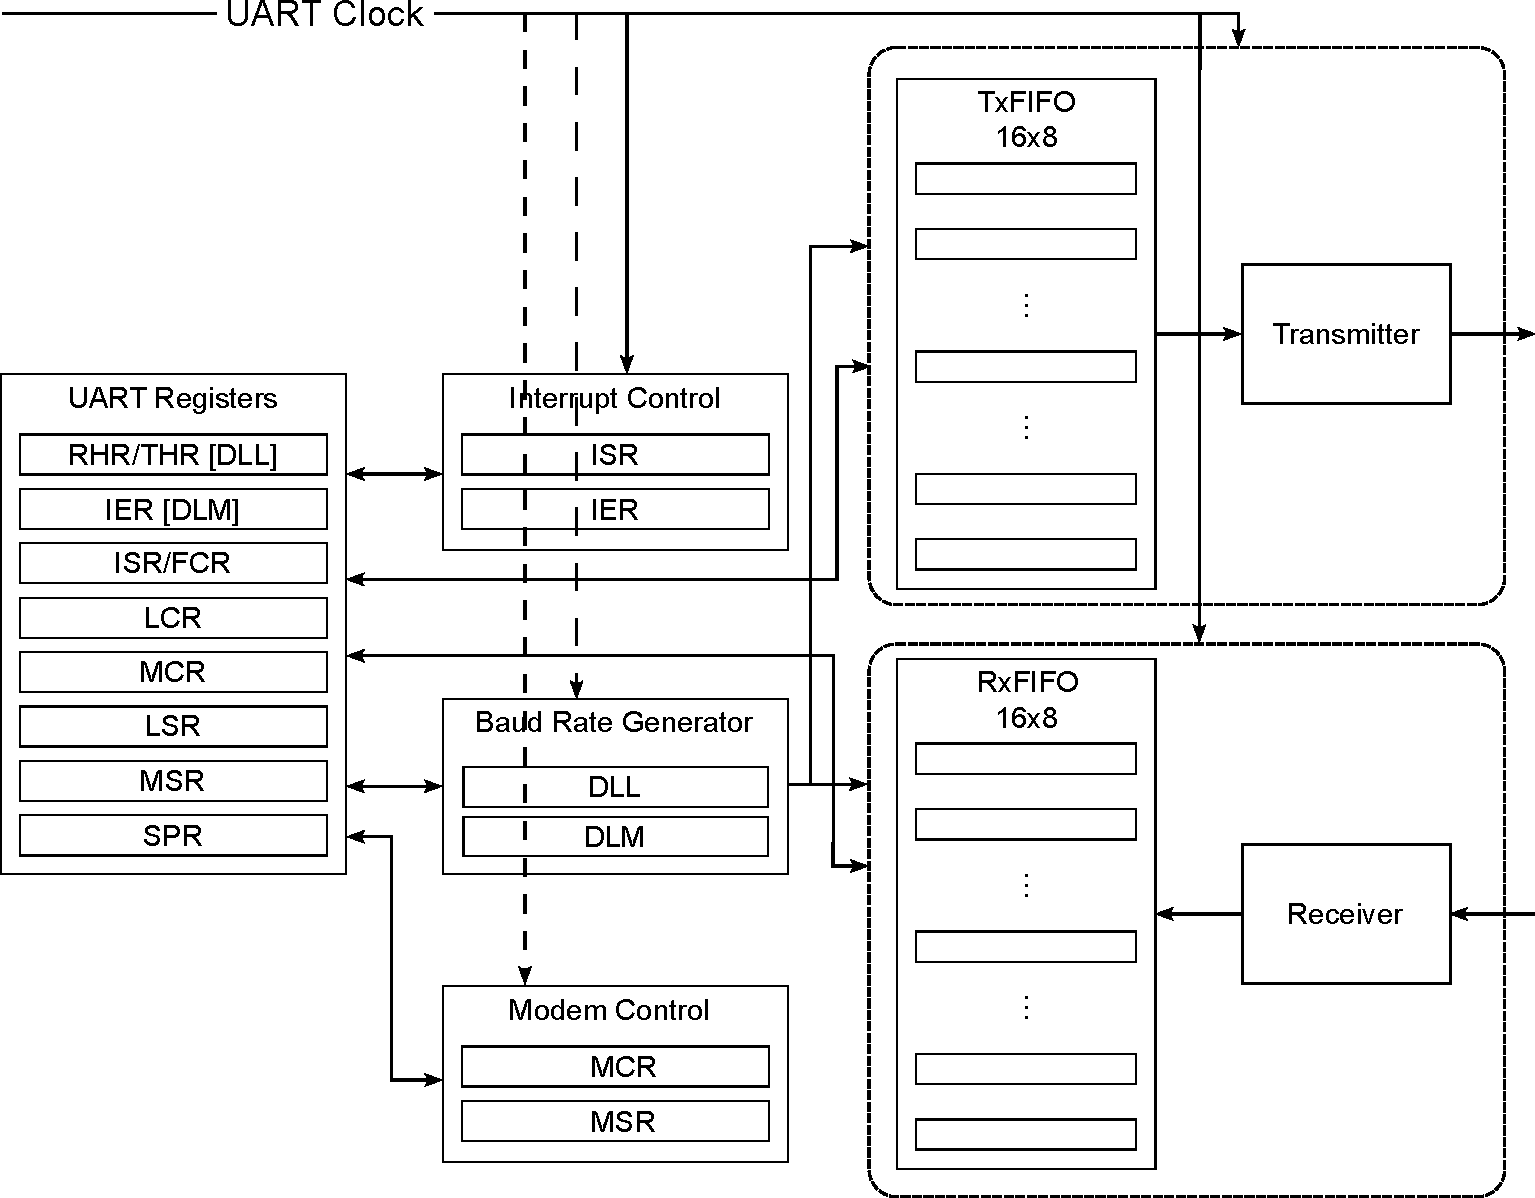
\includegraphics[width=0.85\textwidth]{figures/uart_blk.pdf}
  \caption{UART module high level schematic.}
  \label{fig:obi-uart-schematic}
\end{figure}
The configurator allows the user to add UART modules to either the peripheral cluster in the Pico subsystem or as a part of the NoC subsystem. It is connects to the AHB bus over an AHB to APB bridge that might be shared with any other peripherals in the cluster. \todo{Fix the which UART is used for the NoC sys.}

Both modules provide optional modem control pins as listed in \autoref{tab:uart-modem-signal-list}. 
\begin{table}[htbp]
  \centering
  \begin{tabular}{r l}
    \toprule 
    Signal & Function\footnote{I = Input, O = Output} \\
    \midrule 
    \texttt{cts\_n} & Clear to Send (I)\\
    \texttt{dsr\_n} & Data Send Request (I)\\
    \texttt{ri\_n} & Ring Indicator (I)\\
    \texttt{cd\_n} & Carrier Detect (I)\\
    \texttt{rts\_n} & Ready to Send (O) \\
    \texttt{dtr\_n} & Data Ready (O)\\
    \texttt{out1\_n} & GP signal (optional, O)\\
    \texttt{out2\_n} & GP signal (optional, O)\\
    \bottomrule
  \end{tabular}
  \caption{Optional Modem Control Signals available in the UART module.}
  \label{tab:uart-modem-signal-list}
\end{table}
Use of most signals are implied by their names except, perhaps Ring Indicator and Carrier Detect input signals. These signals (all of them in the table above) are a part of the RS232 Interface specification. The two signals in particular are remnants of the dial-up internet/modem era, and can be safely ignored.  

The modules translate the external AXI/APB interface to a register interface. Registers are byte-addressed on 4-byte boundaries. The 3-bit register index is taken from R/W address bits \texttt{addr[4:2]}:

\[
\texttt{byte\_offset} = \texttt{addr[4:2]} \times 4
\]

The absolute base address is defined by the SoC interconnect (for example, \texttt{0x5000.0000} in Libre-V). Offsets in this document are relative to the UART instance base.

\section{Using the UART}

\subsection{DLAB (Divisor Latch Access Bit)}

Bit~7 of the Line Control Register (\textbf{LCR.DLAB}) multiplexes the mapping at offsets
\texttt{0x00} and \texttt{0x04}:

\begin{itemize}[nosep]
  \item \textbf{DLAB = 0}: normal operation (data and interrupt enable registers).
  \item \textbf{DLAB = 1}: baud-rate divisor latches (\textbf{DLL}, \textbf{DLM}).
\end{itemize}

\subsection{Setting the operating Baud Rate}
To set the baud rate, find the baud rate divisor using:
\[
\mathrm{Divisor} = \frac{\mathrm{SysClkFreq\ (in\ Hz)}}{16 \times \mathrm{Baud\ Rate}}.
\] 
Having found the divisor, you need to quantize it to 16-bits\footnote{The UART currently only supports integer divisors.}. The design generates train of enable pulses based of the provided clock (as opposed to actually dividing the clock signal) based on this divisor. 

To configure the UART, enable the divisor latches by setting \textbf{DLAB = 1}, and set the least significant byte of the 16-bit divisor in \textbf{DLL} and the most significant byte in \textbf{DLM}. 

\subsection{Read/Write Shared Addresses}

Several register names share the same byte offset. The hardware distinguishes them by the
bus transaction direction (\texttt{a.we}):

\begin{itemize}[nosep]
  \item A \textbf{read} at offset \texttt{0x00} returns \textbf{RHR}; a \textbf{write}
        stores \textbf{THR} (when DLAB = 0).
  \item A \textbf{read} at offset \texttt{0x08} returns \textbf{ISR}; a \textbf{write}
        updates \textbf{FCR}.
\end{itemize}

\subsection{FIFOs}

When \textbf{FCR.FIFO\_EN} is set, the transmit and receive paths each use a 16-entry FIFO.
When cleared, only a single-byte holding register is available on each path.

\section{Register Descriptions} 
The following section describes the UART registers in the numerical order of address offset. This section will be useful for those wanting to write custom UART drivers or understand/debug existing drivers. 

\regtitle{0}{Receiver Holding Register (RHR) / Transmitter Holding Register (THR)}

\regmeta{SoC-defined}{0x000}{0x00}{RHR -- RO; THR -- WO}{Read-sensitive (RHR). DLAB must be 0.}

\begin{register}{H}{UART Data Registers RHR/THR}{}

  \regfield[gray!20]{Reserved}{24}{8}{{uninitialized}}
  \regfield{DATA}{8}{0}{00000000}
  \reglabel{Reset}

  \regfieldvalue[gray!20]{Reserved}{24}{8}{{RO}}
  \regfieldvalue{DATA}{8}{0}{{RW}}
  \reglabel{Type}

\end{register}


\textbf{Functional Description.}

Offset \texttt{0x000} is shared by the Receiver Holding Register and the Transmitter Holding Register. A read returns the oldest received data byte from the receive FIFO (if enabled) or from the single-byte RHR. A write pushes a transmit data byte into the transmit FIFO (if enabled) or into the THR; transmission begins automatically when the transmitter is idle.

When DLAB = 1, this offset maps to the Divisor Latch LSB (\textbf{DLL}) instead; see Register~10.

\begin{regmap}
7:0 & DATA & RHR: RO\newline THR: WO & 0 &
Receive/transmit data byte. On read, returns the received character.
On write, loads the next character to transmit. \\
\end{regmap}


\regtitle{1}{Interrupt Enable Register (IER)}

\regmeta{SoC-defined}{0x004}{0x00}{RW}{DLAB must be 0. When DLAB = 1, this offset maps to DLM.}

\begin{register}{H}{UART Intterupt Enable Register (IER)}{}
 
  \regfield[gray!20]{Reserved}{28}{4}{{0}}
  \regfield{MSTAT}{1}{3}{0}
  \regfield{RLTAT}{1}{2}{0}
  \regfield{THRE}{1}{1}{0}
  \regfield{DR}{1}{0}{0}
  \reglabel{Reset}
 
  \regfieldvalue[gray!20]{Reserved}{28}{4}{{RW}}
  \regfieldvalue{MSTAT}{1}{3}{RW}
  \regfieldvalue{RLTAT}{1}{2}{RW}
  \regfieldvalue{THRE}{1}{1}{RW}
  \regfieldvalue{DR}{1}{0}{RW}  
  \reglabel{Type}
 
\end{register}


\textbf{Functional Description.}

The Interrupt Enable Register masks individual interrupt sources. A bit set to 1 allows the
corresponding condition to contribute to the interrupt output \texttt{irq\_o}. Reading or
writing IER does not clear pending interrupts.

\begin{regmap}
7:4 & reserved & RO & 0 &
Reserved. Read as 0. Writes are stored but have no effect. \\
3 & MSTAT & RW & 0 &
Modem Status interrupt enable. When 1, a change in modem status lines may assert an interrupt. \\
2 & RLSTAT & RW & 0 &
Receive Line Status interrupt enable. When 1, overrun, parity, framing, or break errors may
assert an interrupt. \\
1 & THRE & RW & 0 &
Transmitter Holding Register Empty interrupt enable. When 1, an empty THR/TX FIFO may assert
an interrupt. \\
0 & DR & RW & 0 &
Data Ready / Reception Timeout interrupt enable. When 1, received data available or a character
timeout (FIFO mode) may assert an interrupt. \\
\end{regmap}

\regtitle{2}{Interrupt Status Register (ISR)}

\regmeta{SoC-defined}{0x008}{0xC1}{RO}{Read-only. DLAB must be 0.}

\begin{register}{H}{UART Interrupt Status Register (ISR)}{}
 
  \regfield[gray!20]{Reserved}{24}{8}{{0}}
  \regfield{FIFOS\_EN}{2}{6}{11}
  \regfield[gray!20]{Reserved}{2}{4}{{0}}
  \regfield{ID}{3}{1}{000}
  \regfield{STATUS}{1}{0}{1}
  \reglabel{Reset}
 
  \regfieldvalue[gray!20]{Reserved}{24}{8}{{RO}}
  \regfieldvalue{FIFOS\_EN}{2}{6}{{RO}}
  \regfieldvalue[gray!20]{Reserved}{2}{4}{{RO}}
  \regfieldvalue{ID}{3}{1}{{RO}}
  \regfieldvalue{STATUS}{1}{0}{{RO}}
  \reglabel{Type}
 
\end{register}

\textbf{Functional Description.}

The Interrupt Status Register reports whether an interrupt is pending and, if so, the highest
priority interrupt source. The register is implemented in \texttt{obi\_uart\_interrupts.sv}
and is not stored in the main register flip-flop array. Reading ISR identifies the interrupt source but does not by itself clear all interrupt conditions; associated status registers (LSR, MSR, RHR) may need to be serviced.

\begin{regmap}
7:6 & FIFOS\_EN & RO & 2'b11 &
FIFO capability field. Hardwired to \texttt{2'b11} to indicate 16550A-style FIFO support. \\
5:4 & reserved  & RO & 0   & Reserved. Read as 0. \\
3:1 & ID        & RO & 0   &
Interrupt identification code when \textbf{STATUS} = 0:
\begin{itemize}[nosep,leftmargin=*]
  \item \texttt{011}: Receive line status
  \item \texttt{010}: Received data available
  \item \texttt{110}: Character timeout (FIFO mode)
  \item \texttt{001}: THR empty
  \item \texttt{000}: Modem status
\end{itemize} \\
0   & STATUS    & RO & 1   &
Interrupt status. 0 = interrupt pending; 1 = no interrupt pending. \\
\end{regmap}
The ID field is updated in the priority encoder in the interrupt submodule. 

\regtitle{3}{FIFO Control Register (FCR)}

\regmeta{SoC-defined}{0x008}{0x00}{WO}{Write-only. Shares offset with ISR.}

\begin{register}{H}{UART FIFO Control Register (FCR)}{}
 
  \regfield[gray!20]{Reserved}{24}{8}{{0}}
  \regfield{RX\_FIFO\_TL}{2}{6}{00}
  \regfield[gray!20]{Reserved}{3}{3}{{0}}
  \regfield{TX\_FIFO\_RST}{1}{2}{0}
  \regfield{RX\_FIFO\_RST}{1}{1}{0}
  \regfield{FIFO\_EN}{1}{0}{0}
  \reglabel{Reset}
 
  \regfieldvalue[gray!20]{Reserved}{24}{8}{{WO}}
  \regfieldvalue{RX\_FIFO\_TL}{2}{6}{{WO}}
  \regfieldvalue[gray!20]{Reserved}{3}{3}{{WO}}
  \regfieldvalue{TX\_FIFO\_RST}{1}{2}{WO}
  \regfieldvalue{RX\_FIFO\_RST}{1}{1}{WO}
  \regfieldvalue{FIFO\_EN}{1}{0}{WO}
  \reglabel{Type}
 
\end{register}


\textbf{Functional Description.}

The FIFO Control Register configures the on-chip transmit and receive FIFOs that are a part of the UART Tx and Rx submodules. Writes to this
register at offset \texttt{0x008} update FCR; reads at the same offset return ISR.

The RX and TX FIFOs are each 16 entries deep. The RX FIFO stores 11 bits per entry (8 data
bits plus break, framing, and parity error flags). The TX FIFO stores 8-bit characters.

\begin{regmap}
7:6 & RX\_FIFO\_TL      & WO & 0 &
Receive FIFO trigger level:
\begin{itemize}[nosep,leftmargin=*]
  \item \texttt{00}: 1 character
  \item \texttt{01}: 4 characters
  \item \texttt{10}: 8 characters
  \item \texttt{11}: 14 characters
\end{itemize} \\
5:3 & reserved  & WO & 0 & Reserved. \\
2   & TX\_FIFO\_RST & WO & 0 &
Write 1 to reset/clear the transmit FIFO.\\
1   & RX\_FIFO\_RST & WO & 0 &
Write 1 to reset/clear the receive FIFO.\\
0   & FIFO\_EN  & WO & 0 &
FIFO enable. 0 = 8250-style single-byte THR/RHR; 1 = 16550A 16-byte FIFO mode. \\
\end{regmap}


\regtitle{4}{Line Control Register (LCR)}

\regmeta{SoC-defined}{0x00C}{0x00}{RW}{Accessible regardless of DLAB.}

\begin{register}{H}{UART Line Control Register (LCR)}{}
 
  \regfield[gray!20]{Reserved}{24}{8}{{0}}
  \regfield{DLAB}{1}{7}{0}
  \regfield{SBREAK}{1}{6}{0}
  \regfield{SPAR}{1}{5}{0}
  \regfield{EPAR}{1}{4}{0}
  \regfield{PEN}{1}{3}{0}
  \regfield{STP}{1}{2}{0}
  \regfield{WLS}{2}{0}{00}
  \reglabel{Reset}
 
  \regfieldvalue[gray!20]{Reserved}{24}{8}{{RW}}
  \regfieldvalue{DLAB}{1}{7}{{RW}}
  \regfieldvalue{SBREAK}{1}{6}{{RW}}
  \regfieldvalue{SPAR}{1}{5}{{RW}}
  \regfieldvalue{EPAR}{1}{4}{{RW}}
  \regfieldvalue{PEN}{1}{3}{{RW}}
  \regfieldvalue{STP}{1}{2}{{RW}}
  \regfieldvalue{WLS}{2}{0}{{RW}}
  \reglabel{Type}
 
\end{register}


\textbf{Functional Description.}

The Line Control Register defines the serial frame format and the DLAB address-multiplexing
bit. Changes to word length, parity, and stop bits take effect for subsequently transmitted
and received characters.

\begin{regmap}
7   & DLAB      & RW & 0 &
Divisor Latch Access Bit. When 1, offsets \texttt{0x00} and \texttt{0x04} access DLL and DLM.
When 0, they access RHR/THR and IER. \\
6   & SBREAK    & RW & 0 &
Set Break. When 1, forces the transmit output to a spacing (low) condition. \\
5   & SPAR      & RW & 0 &
Stick Parity. When parity is enabled, forces parity bit to 0 (if EPAR = 1) or 1 (if EPAR = 0). \\
4   & EPAR      & RW & 0 &
Even Parity select. 0 = odd parity; 1 = even parity (when parity enabled). \\
3   & PEN       & RW & 0 &
Parity Enable. When 1, a parity bit is transmitted and checked. \\
2   & STP       & RW & 0 &
Stop Bits. 0 = one stop bit; 1 = two stop bits (1.5 stop bits when word length is 5 bits). \\
1:0 & WLS       & RW & 0 &
Word Length Select:
\begin{itemize}[nosep,leftmargin=*]
  \item \texttt{00}: 5 data bits
  \item \texttt{01}: 6 data bits
  \item \texttt{10}: 7 data bits
  \item \texttt{11}: 8 data bits
\end{itemize} \\
\end{regmap}


\regtitle{5}{Modem Control Register (MCR)}

\regmeta{SoC-defined}{0x010}{0x00}{RW}{Accessible regardless of DLAB.}

\begin{register}{H}{UART Modem Control Register (MCR)}{}
 
  \regfield[gray!20]{Reserved}{24}{8}{{0}}
  \regfield[gray!20]{Reserved}{3}{5}{{0}}
  \regfield{LOOP}{1}{4}{0}
  \regfield{OUT2}{1}{3}{0}
  \regfield{OUT1}{1}{2}{0}
  \regfield{RTS}{1}{1}{0}
  \regfield{DTR}{1}{0}{0}
  \reglabel{Reset}
 
  \regfieldvalue[gray!20]{Reserved}{24}{8}{{RW}}
  \regfieldvalue[gray!20]{Reserved}{3}{5}{{RO}}
  \regfieldvalue{LOOP}{1}{4}{RW}
  \regfieldvalue{OUT2}{1}{3}{RW}
  \regfieldvalue{OUT1}{1}{2}{RW}
  \regfieldvalue{RTS}{1}{1}{RW}
  \regfieldvalue{DTR}{1}{0}{RW}
  \reglabel{Type}
 
\end{register}

\textbf{Functional Description.}

The Modem Control Register drives modem output pins and enables internal loopback for test.
Modem outputs are active-low on the external pins (\texttt{rts\_no}, \texttt{dtr\_no}, etc.).

\begin{regmap}
7:5 & reserved  & RO & 0 & Reserved. Read as 0. \\
4   & LOOP      & RW & 0 &
Loopback. When 1, the transmitter output is looped back to the receiver input internally. \\
3   & OUT2      & RW & 0 & Auxiliary output 2 (optional GPIO). \\
2   & OUT1      & RW & 0 & Auxiliary output 1 (optional GPIO). \\
1   & RTS       & RW & 0 & Request To Send output. \\
0   & DTR       & RW & 0 & Data Terminal Ready output. \\
\end{regmap}

\regtitle{6}{Line Status Register (LSR)}

\regmeta{SoC-defined}{0x014}{0x60}{RO}{Read-sensitive. DLAB must be 0.}

\begin{register}{H}{UART Line Status Register (LSR)}{}
 
  \regfield[gray!20]{Reserved}{24}{8}{{0}}
  \regfield{FIFO\_ERR}{1}{7}{0}
  \regfield{TXE}{1}{6}{1}
  \regfield{THRE}{1}{5}{1}
  \regfield{BI}{1}{4}{0}
  \regfield{FE}{1}{3}{0}
  \regfield{PE}{1}{2}{0}
  \regfield{OE}{1}{1}{0}
  \regfield{DR}{1}{0}{0}
  \reglabel{Reset}
 
  \regfieldvalue[gray!20]{Reserved}{24}{8}{{RO}}
  \regfieldvalue{FIFO\_ERR}{1}{7}{RO}
  \regfieldvalue{TXE}{1}{6}{RO}
  \regfieldvalue{THRE}{1}{5}{RO}
  \regfieldvalue{BI}{1}{4}{RO}
  \regfieldvalue{FE}{1}{3}{RO}
  \regfieldvalue{PE}{1}{2}{RO}
  \regfieldvalue{OE}{1}{1}{RO}
  \regfieldvalue{DR}{1}{0}{RO}
  \reglabel{Type}
 
\end{register}


\textbf{Functional Description.}

The Line Status Register provides transmit readiness and receive status, including error
flags. Unlike some UART designs, error information is \emph{not} embedded in the RHR read
data; errors are reported only in LSR. Reading LSR clears the receive-line-status interrupt. Individual error bits are cleared on
LSR read when no additional FIFO errors remain.

\begin{regmap}
7   & FIFO\_ERR   & RO & 0 &
FIFO Error. Set when at least one character with an error was received into the RX FIFO. \\
6   & TXE    & RO & 1 &
Transmitter Empty. 1 when the transmitter shift register and holding logic are completely idle. \\
5   & THRE    & RO & 1 &
THR Empty. 1 when the THR or TX FIFO can accept a new write. \\
4   & BI      & RO & 0 &
Break Indicator. 1 when a break condition was detected on the receive line. \\
3   & FE      & RO & 0 &
Framing Error. 1 when the stop bit was not received as expected. \\
2   & PE      & RO & 0 &
Parity Error. 1 when the received parity bit did not match. \\
1   & OE      & RO & 0 &
Overrun Error. 1 when a new character arrived before the previous one was read (RHR mode) or
when the RX FIFO was full (FIFO mode). \\
0   & DR      & RO & 0 &
Data Ready. 1 when received data is available in RHR or the RX FIFO. \\
\end{regmap}


\regtitle{7}{Modem Status Register (MSR)}

\regmeta{SoC-defined}{0x018}{0x00}{RO}{Read-sensitive. DLAB must be 0.}

\begin{register}{H}{UART Modem Status Register (MSR)}{}
 
  \regfield[gray!20]{Reserved}{24}{8}{{0}}
  \regfield{CD}{1}{7}{0}
  \regfield{RI}{1}{6}{0}
  \regfield{DSR}{1}{5}{0}
  \regfield{CTS}{1}{4}{0}
  \regfield{DCD}{1}{3}{0}
  \regfield{TERI}{1}{2}{0}
  \regfield{DDSR}{1}{1}{0}
  \regfield{DCTS}{1}{0}{0}
  \reglabel{Reset}
 
  \regfieldvalue[gray!20]{Reserved}{24}{8}{{RO}}
  \regfieldvalue{CD}{1}{7}{RO}
  \regfieldvalue{RI}{1}{6}{RO}
  \regfieldvalue{DSR}{1}{5}{RO}
  \regfieldvalue{CTS}{1}{4}{RO}
  \regfieldvalue{DCD}{1}{3}{RO}
  \regfieldvalue{TERI}{1}{2}{RO}
  \regfieldvalue{DDSR}{1}{1}{RO}
  \regfieldvalue{DCTS}{1}{0}{RO}
  \reglabel{Type}
 
\end{register}


\textbf{Functional Description.}

The Modem Status Register reports the state of modem input signals and edge-detected changes.
Delta bits (bits 4--7 in this implementation) are sticky and remain set until MSR is read.

Modem input pins are active-low externally; the register stores the logical (non-inverted)
levels and change indicators.

\begin{regmap}
7   & CD    & RO & 0 & Carrier Detect input level. \\
6   & RI    & RO & 0 & Ring Indicator input level. \\
5   & DSR   & RO & 0 & Data Set Ready input level. \\
4   & CTS   & RO & 0 & Clear To Send input level. \\
3   & DCD  & RO & 0 & Delta Carrier Detect. Set when CD input changes state. \\
2   & TERI  & RO & 0 & Trailing Edge Ring Indicator. Set on high-to-low transition of RI. \\
1   & DDSR  & RO & 0 & Delta Data Set Ready. Set when DSR input changes state. \\
0   & DCTS  & RO & 0 & Delta Clear To Send. Set when CTS input changes state. \\
\end{regmap}


\regtitle{8}{Scratch Pad Register (SPR)}

\regmeta{SoC-defined}{0x01C}{0x00}{RO}{Not implemented.}

\begin{register}{H}{UART Scratch Pad Register (SPR)}{}
 
  \regfield[gray!20]{Reserved}{24}{8}{{0}}
  \regfield{DATA}{8}{0}{00000000}
  \reglabel{Reset}
 
  \regfieldvalue[gray!20]{Reserved}{24}{8}{{RO}}
  \regfieldvalue{DATA}{8}{0}{{RO}}
  \reglabel{Type}
 
\end{register}


\textbf{Functional Description.}

The optional Scratch Pad Register is defined by the 16550A standard as a software-writable storage
location. In this implementation, reads always return \texttt{0x00} and writes are silently
ignored. No error is generated.

\begin{regmap}
7:0 & DATA & RO & 0 & Always reads zero. Writes have no effect. \\
\end{regmap}


\regtitle{9}{Divisor Latch LSB (DLL)}

\regmeta{SoC-defined}{0x000}{0x01}{RW}{DLAB must be 1. Shares offset with RHR/THR.}

\begin{register}{H}{UART Divisor Latch LSB (DLL)}{}
 
  \regfield[gray!20]{Reserved}{24}{8}{{uninitialized}}
  \regfield{DIV\_LSB}{8}{0}{00000001}
  \reglabel{Reset}
 
  \regfieldvalue[gray!20]{Reserved}{24}{8}{{RO}}
  \regfieldvalue{DIV\_LSB}{8}{0}{{RW}}
  \reglabel{Type}
 
\end{register}


\textbf{Functional Description.}

When DLAB = 1, offset \texttt{0x000} maps to the least significant byte of the 16-bit baud
rate divisor. The divisor is combined with DLM as:

% \[
% \mathrm{divisor} = \{\mathrm{DLM}, \mathrm{DLL}\}, \qquad
% \mathrm{baud} = \frac{f_{\mathrm{clk}}}{16 \times \mathrm{divisor}}
% \]

A divisor of 0 is invalid and disables baud-rate generation. Writing DLL or DLM resets the
internal baud counters.

\begin{regmap}
7:0 & DIV\_LSB & RW & 0x01 & Least significant byte of the baud divisor latch. \\
\end{regmap}


\regtitle{10}{Divisor Latch MSB (DLM)}

\regmeta{SoC-defined}{0x004}{0x00}{RW}{DLAB must be 1. Shares offset with IER.}

\begin{register}{H}{UART Divisor Latch MSB (DLM)}{}
  \regfield[gray!20]{Reserved}{24}{8}{{0}}
  \regfield{DIV\_MSB}{8}{0}{00000000}
  \reglabel{Reset}
  \regfieldvalue[gray!20]{Reserved}{24}{8}{{RW}}
  \regfieldvalue{DIV\_MSB}{8}{0}{{RW}}
  \reglabel{Type}

\end{register}


\textbf{Functional Description.}

When DLAB = 1, offset \texttt{0x004} maps to the most significant byte of the baud rate
divisor. See Register~9 for the baud-rate formula.

\begin{regmap}
7:0 & DIV\_MSB & RW & 0x00 & Most significant byte of the baud divisor latch. \\
\end{regmap}


\subsection{Address Map Summary}

\begin{tabular}{@{}lllll@{}}
\toprule
\textbf{Offset} & \textbf{DLAB = 0 (read)} & \textbf{DLAB = 0 (write)} &
\textbf{DLAB = 1 (read)} & \textbf{DLAB = 1 (write)} \\
\midrule
0x000 & RHR & THR & DLL & DLL \\
0x004 & IER & IER & DLM & DLM \\
0x008 & ISR & FCR & ISR & FCR \\
0x00C & LCR & LCR & LCR & LCR \\
0x010 & MCR & MCR & MCR & MCR \\
0x014 & LSR & --- & --- & --- \\
0x018 & MSR & --- & --- & --- \\
0x01C & SPR & SPR & SPR & SPR \\
\bottomrule
\end{tabular}

\newpage

\chapter{Timer Family}\label{ch:sw-timer}

Libre-V offers three different timer options: \begin{enumerate}
  \item \hyperref[sec:sw-basic-timer]{Basic Timer}
  \item General Purpose Timer 
  \item Advanced Timer/PWM
\end{enumerate}

These timer variants differ in their functionality. The feature set increases in the order listed above. All modules are memory mapped APB peripherals.

\section{Basic Timer (BTimer)}\label{sec:sw-basic-timer}

The BTimer module is the ``APB timer'' from the PULP platform. It is a free-running 32-bit up-counter with a programmable clock prescaler and a compare register, and it raises two physical\footnote{By physical we mean that the interrupts are exposed as output ports as opposed to updating registers. These interrupts are made software-readable by connecting it to interrupt ports of the cores either pico or rocket.} interrupts: a counter \emph{overflow} and a \emph{compare match}. 

Note that the BTimer module can instantiate several \texttt{timer} cores behind an internal APB address mux (selected by \texttt{PADDR}). See \autoref{fig:timer-schematic} for a high level view of the module.
\begin{figure}[htbp]
  \centering
  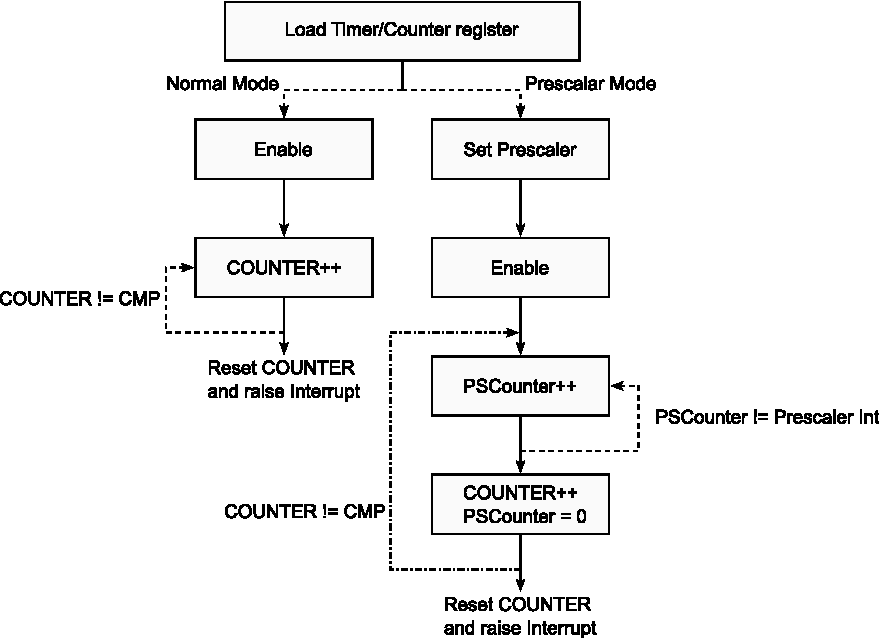
\includegraphics[width=0.85\textwidth]{figures/btimer_flow.pdf}
  \caption{Btimer control flow}
  \label{fig:btimer-flow}
\end{figure}

The Btimer core exposes three 32-bit registers. They are byte-addressed on 4-byte boundaries; the
register index is taken from APB address bits \texttt{PADDR[3:2]}:
\[
\texttt{byte\_offset} = \texttt{PADDR[3:2]} \times 4
\]

\begin{docnote}
  The base address of a Btimer can be found in the generated software library file(s) as these depend on the user-specific configuration. Offsets in this document are relative to the timer instance base.
\end{docnote}

\section*{Using the Btimer}

Figure~\autoref{fig:btimer-flow} illustrates the control flow of the Btimer module. 

\subsection{Counting and the Prescaler}

When \textbf{CTRL.EN} is set, the counter advances at a rate governed by the 3-bit prescaler field
\textbf{CTRL.PSC}. A free-running \emph{cycle counter} counts input clock cycles from \texttt{0} up
to the prescaler value and then wraps:
\begin{itemize}[nosep]
  \item \textbf{PSC = 0} (normal mode): the counter increments on every clock cycle.
  \item \textbf{PSC $\neq$ 0} (prescaled mode): the counter increments once every
        $(\mathrm{PSC}+1)$ clock cycles.
\end{itemize}
So the effective counting rate is $f_{\mathrm{clk}} / (\mathrm{PSC}+1)$.

\subsection{Compare, Overflow, and Auto-reset}

The counter is compared against the \textbf{CMP} register on each tick:
\begin{itemize}[nosep]
  \item \textbf{Compare match}: when \texttt{CMP} $\neq 0$ and the counter equals \texttt{CMP}, the
        compare-match interrupt (\texttt{irq\_o[1]}) is asserted and the counter is reset to
        \texttt{0}. A \texttt{CMP} value of \texttt{0} disables the compare function.
  \item \textbf{Overflow}: when the counter reaches \texttt{0xFFFF\_FFFF} and the next tick occurs,
        the overflow interrupt (\texttt{irq\_o[0]}) is asserted and the counter wraps to \texttt{0}.
\end{itemize}
Both interrupts are single-cycle pulses generated combinationally on the tick. In addition,
\emph{writing} the \texttt{CMP} register resets the counter to \texttt{0}, which makes it easy to
start a fresh timed interval. This gives a straightforward periodic-tick usage: program a prescaler
and a compare value, enable the timer, and take a compare-match interrupt every
$(\mathrm{CMP}+1)\times(\mathrm{PSC}+1)$ clock cycles.

\subsection{Register Descriptions}
The following section describes the TIMER registers in the numerical order of address offset.

\regtitle{0}{Timer Counter Register (TIMER)}

\regmeta{SoC-defined}{0x000}{0x00}{RW}{Free-running count. Auto-resets on match/overflow/CMP write.}

\begin{register}{H}{Timer Counter Register (TIMER)}{}

  \regfield{COUNT}{32}{0}{{00000000000000000000000000000000}}
  \reglabel{Reset}

  \regfieldvalue{COUNT}{32}{0}{{RW}}
  \reglabel{Type}

\end{register}

\textbf{Functional Description.}

Offset \texttt{0x000} holds the current 32-bit counter value. A read returns the instantaneous
count. A write preloads the counter, allowing software to start from an arbitrary value. When the
timer is enabled the hardware advances this register at the prescaled rate, and clears it to
\texttt{0} on a compare match, on overflow, or when the \textbf{CMP} register is written.

\begin{regmap}
31:0 & COUNT & RW & 0 &
Current timer count. Readable at any time; a write preloads the counter. Advances at
$f_{\mathrm{clk}}/(\mathrm{PSC}+1)$ while \textbf{CTRL.EN} = 1. \\
\end{regmap}

\regtitle{1}{Timer Control Register (CTRL)}

\regmeta{SoC-defined}{0x004}{0x00}{RW}{Only EN (bit 0) and PSC (bits 5:3) are functional.}

\begin{register}{H}{Timer Control Register (CTRL)}{}

  \regfield[gray!20]{Reserved}{26}{6}{{0}}
  \regfield{PSC}{3}{3}{000}
  \regfield[gray!20]{Reserved}{2}{1}{{0}}
  \regfield{EN}{1}{0}{0}
  \reglabel{Reset}

  \regfieldvalue[gray!20]{Reserved}{26}{6}{{RW}}
  \regfieldvalue{PSC}{3}{3}{{RW}}
  \regfieldvalue[gray!20]{Reserved}{2}{1}{{RW}}
  \regfieldvalue{EN}{1}{0}{{RW}}
  \reglabel{Type}

\end{register}

\textbf{Functional Description.}

The Control Register enables the counter and sets the prescaler. The full 32-bit word is stored, so
the reserved bits are writable and read back their last written value, but they have no effect on
operation.

\begin{regmap}
31:6 & reserved & RW & 0 &
Reserved. Stored but have no effect. \\
5:3  & PSC      & RW & 0 &
Prescaler. The counter increments once every $(\mathrm{PSC}+1)$ clock cycles. \texttt{PSC = 0}
selects normal mode (increment every cycle). \\
2:1  & reserved & RW & 0 &
Reserved. Stored but have no effect. \\
0    & EN       & RW & 0 &
Enable. When 1, the counter runs; when 0, the counter is frozen at its current value. \\
\end{regmap}

\regtitle{2}{Timer Compare Register (CMP)}

\regmeta{SoC-defined}{0x008}{0x00}{RW}{Writing CMP resets the counter to 0. CMP = 0 disables compare.}

\begin{register}{H}{Timer Compare Register (CMP)}{}

  \regfield{CMP}{32}{0}{{0}}
  \reglabel{Reset}

  \regfieldvalue{CMP}{32}{0}{{RW}}
  \reglabel{Type}

\end{register}

\textbf{Functional Description.}

Offset \texttt{0x008} holds the 32-bit compare value. When the counter reaches this value (and the
value is non-zero), the compare-match interrupt \texttt{irq\_o[1]} is asserted and the counter is
reset to \texttt{0}, producing a periodic tick of period $(\mathrm{CMP}+1)\times(\mathrm{PSC}+1)$ clock
cycles. Writing this register also immediately resets the counter to \texttt{0}, so software should
program \textbf{CMP} before starting the count. A value of \texttt{0} disables the compare path,
leaving only the overflow interrupt active.

\begin{regmap}
31:0 & CMP & RW & 0 &
Compare value. On \texttt{COUNT == CMP} (with \texttt{CMP} $\neq 0$) the compare-match interrupt
fires and the counter clears. Writing this field also clears the counter. \texttt{CMP = 0}
disables the compare match. \\
\end{regmap}

\subsection{Interrupts}

The timer core drives a 2-bit interrupt output \texttt{irq\_o[1:0]}:

\begin{tabular}{@{}cll@{}}
\toprule
\textbf{Bit} & \textbf{Name} & \textbf{Condition} \\
\midrule
0 & Overflow      & Counter wraps from \texttt{0xFFFF\_FFFF}. \\
1 & Compare match & Counter equals a non-zero \texttt{CMP}. \\
\bottomrule
\end{tabular}

\subsection{Address Map Summary}

\begin{tabular}{@{}lll@{}}
\toprule
\textbf{Offset} & \textbf{Register} & \textbf{Access} \\
\midrule
0x000 & TIMER (counter) & RW \\
0x004 & CTRL (control)  & RW \\
0x008 & CMP (compare)   & RW \\
\bottomrule
\end{tabular}

% \section{APB Advanced Timer} 

% Sourced from OpenHW Group's Core-V-MCU\footnote{\href{https://docs.openhwgroup.org/projects/core-v-mcu/doc-src/ip-blocks/apb_adv_timer.html}{https://docs.openhwgroup.org/projects/core-v-mcu/doc-src/ip-blocks/apb\_adv\_timer.html}}, the APB Advanced Timer (AAT) is capable of generating PWM for external devices. A single AAT module contains 4 independent, configurable/programmable 16-bit timer modules. 

% \subsection*{Features} 
% \begin{itemize}
%   \item Dual clock source design (APB interface clock + independent clock).
%   \item Multiple input sources: PWM/GPIO.
%   \item Configurable input trigger modes for each timer
%   \item Configurable prescaler for each timer 
%   \item Configurable counting mode for each timer 
%   \item Four comparators for each timer. 
%   \item Configurable channel comparator threshold and comparator operation for each comparator. 
%   \item Four configurable output events 4-bit PWM output for each timer. 
%   \item Configurable clock gating of each timer
% \end{itemize}

% \subsection{Block architecture} 

% Each of the four 16-bit timer is organized as an input stage, prescaler, up-down counter, and comparators. To enable MMIO integration, each of these includes a set of control registers. 

% Each of the APB Timer can generate 4-bit PWM signals (we can have 4 such 4-bit PWMs due to indepedence of all the timer modules). A 4-bit output event can be generated by configuring the \texttt{EVENT\_CFG} register. 

% \begin{figure}[htbp]
%   \centering
%   
\includegraphics[width=0.95\textwidth]{figures/tmp/apb_adv_timer_block_diagram.png}
%   \caption{APB Advanced Timer block diagram.}
%   \label{fig:apb-adv-timer-blk}
% \end{figure}

% \begin{figure}[htbp]
%   \centering
%   
\includegraphics[width=0.95\textwidth]{figures/tmp/apb_adv_timer_diagram_1.png}
%   \caption{APB Timer (child module) block diagram.}
%   \label{fig:apb-adv-timer-blk-tmp}
% \end{figure}

% \subsubsection{Timer Module}


% % \section{Overview}


% % \subsection{Source Files}

% % \begin{tabular}{@{}ll@{}}
% % \toprule
% % \textbf{File} & \textbf{Role} \\
% % \midrule
% % \texttt{apb\_timer/src/timer.sv}          & Single timer core: counter, prescaler, compare, IRQs \\
% % \texttt{apb\_timer/src/apb\_timer.sv}     & Multi-timer APB wrapper with internal address mux \\
% % \texttt{apb\_timer/src/apb\_timer\_wrap.sv} & Struct-to-flat APB wrapper around one \texttt{timer} core \\
% % \texttt{axi\_timer/axi\_timer.sv}         & NoC-side AXI4 $\rightarrow$ APB adapter chain \\
% % \bottomrule
% % \end{tabular}

% % \newpage


% \newpage
% \chapter{Direct Memory Access (DMA)}\label{ch:sw-dma}

\section{Overview}
Libre-V includes a single-channel DMA engine built from the PULP platform's \texttt{iDMA}. It is a NoC
manager \emph{and} a NoC subordinate: the register frontend is a subordinate endpoint that software
programs (\texttt{0x2020\_0000} in Libre-V), while the datapath is a separate manager endpoint
(\texttt{dma\_mngr}) that issues the AXI4 read/write bursts moving the data. Both cores can program it
over the NoC.

The engine is assembled from three iDMA layers:
\begin{enumerate}[nosep]
  \item \textbf{Frontend} --- \texttt{idma\_reg32\_3d}: the 32-bit register file described here. One
        register set (one stream) is instantiated, so only stream~0 of the \texttt{STATUS} /
        \texttt{NEXT\_ID} / \texttt{DONE\_ID} groups is wired; the others read as zero.
  \item \textbf{Midend} --- \texttt{idma\_nd\_midend}: expands a multi-dimensional (1-D/2-D/3-D)
        descriptor into a stream of contiguous transfers.
  \item \textbf{Backend} --- the \texttt{rw\_axi} backend: performs the actual AXI4 bursts. This build
        generates the AXI backend only, so both source and destination protocols must stay AXI.
\end{enumerate}

\subsection{Programming Model}
A transfer is described by writing the address, length, and (for 2-D/3-D) stride/repeat registers, then
\textbf{reading} the \texttt{NEXT\_ID} register. The read is what launches the transfer; it returns the
newly allocated transfer id. Completion is observed by polling \texttt{DONE\_ID} (the last completed id)
or the \texttt{STATUS} busy bits. The typical sequence is:
\begin{enumerate}[nosep]
  \item Program \texttt{CONF} for the number of dimensions and burst options.
  \item Write \texttt{SRC\_ADDR}, \texttt{DST\_ADDR}, \texttt{LENGTH} (and the dimension-2/3 stride and
        repeat registers if applicable).
  \item Read \texttt{NEXT\_ID} to launch; keep the returned id.
  \item Wait until \texttt{DONE\_ID} $\ge$ that id, or until \texttt{STATUS} clears.
\end{enumerate}

\begin{docnote}
Reading \texttt{NEXT\_ID} has a side effect: it \emph{launches} the transfer and increments the id. Do
not read it to ``peek'' at the next id. A returned id of \texttt{0} means the descriptor was not
accepted.
\end{docnote}

\section{Register Descriptions}
Offsets are relative to the DMA frontend base. Only the registers used by the single instantiated
stream are listed; the frontend reserves further offsets for additional streams that are not wired in
this build.

\regtitle{--}{Configuration Register (CONF)}

\regmeta{0x2020\_0000}{0x000}{0x00000000}{RW}{Per-transfer options; program before launching.}

\begin{register}{H}{Configuration Register (CONF)}{}

  \regfield[gray!20]{Reserved}{14}{18}{{0}}
  \regfield{DST\_PROT}{3}{15}{{000}}
  \regfield{SRC\_PROT}{3}{12}{{000}}
  \regfield{ENABLE\_ND}{2}{10}{{00}}
  \regfield{DST\_MLEN}{3}{7}{{000}}
  \regfield{SRC\_MLEN}{3}{4}{{000}}
  \regfield{DRL}{1}{3}{0}
  \regfield{SRL}{1}{2}{0}
  \regfield{DEC\_RW}{1}{1}{0}
  \regfield{DEC\_AW}{1}{0}{0}
  \reglabel{Reset}

\end{register}

\textbf{Functional Description.}

\texttt{CONF} selects the number of active dimensions and tunes burst behaviour. In the base
configuration both protocol fields must remain \texttt{0} (AXI), since only the \texttt{rw\_axi} backend
is generated.

\begin{regmap}
31:18 & reserved   & RW & 0 & Reserved. \\
17:15 & DST\_PROT  & RW & 0 & Destination protocol (\texttt{idma\_pkg::protocol\_e}). Must be 0 (AXI). \\
14:12 & SRC\_PROT  & RW & 0 & Source protocol. Must be 0 (AXI). \\
11:10 & ENABLE\_ND & RW & 0 & Active dimensions: 0 = 1-D, 1 = 2-D, 2 = 3-D. \\
9:7   & DST\_MLEN  & RW & 0 & $\log_2$ of the maximum destination burst length (with \textbf{DRL}). \\
6:4   & SRC\_MLEN  & RW & 0 & $\log_2$ of the maximum source burst length (with \textbf{SRL}). \\
3     & DRL        & RW & 0 & Destination reduce-length: cap destination bursts to \textbf{DST\_MLEN}. \\
2     & SRL        & RW & 0 & Source reduce-length: cap source bursts to \textbf{SRC\_MLEN}. \\
1     & DEC\_RW    & RW & 0 & Fully decouple reads and writes (deadlock risk; use with care). \\
0     & DEC\_AW    & RW & 0 & Issue write addresses only after the first read returns. \\
\end{regmap}

\regtitle{--}{Status Register (STATUS)}

\regmeta{0x2020\_0000}{0x004}{0x00000000}{RO}{Busy bits for the backend sub-units and the midend.}

\textbf{Functional Description.}

\texttt{STATUS} is the packed busy vector \{\,\texttt{midend\_busy}, \texttt{idma\_busy}\,\}: bits
\texttt{[7:0]} are the backend sub-unit busy flags and bit~8 is the ND midend. The engine is idle when
the whole field reads \texttt{0}.

\begin{regmap}
8   & MIDEND\_BUSY & RO & 0 & ND midend is expanding a descriptor. \\
7:0 & IDMA\_BUSY   & RO & 0 & Backend busy flags: buffer, R/W datapath, R/W legalizer, error handler, RAW coupler. \\
\end{regmap}

\regtitle{--}{Next-ID Register (NEXT\_ID)}

\regmeta{0x2020\_0000}{0x044}{0x00000000}{RO}{Reading launches the transfer and returns the new id.}

\textbf{Functional Description.}

Reading \texttt{NEXT\_ID} commits the currently programmed descriptor and returns its transfer id.
A return value of \texttt{0} indicates the descriptor was rejected.

\begin{regmap}
31:0 & NEXT\_ID & RO & 0 & Read to launch; returns the allocated id (0 = rejected). \\
\end{regmap}

\regtitle{--}{Done-ID Register (DONE\_ID)}

\regmeta{0x2020\_0000}{0x084}{0x00000000}{RO}{Id of the most recently completed transfer.}

\textbf{Functional Description.}

\texttt{DONE\_ID} holds the id of the last completed transfer. A transfer with id $n$ has finished once
\texttt{DONE\_ID} $\ge n$.

\begin{regmap}
31:0 & DONE\_ID & RO & 0 & Last completed transfer id. \\
\end{regmap}

\subsection{Descriptor Registers}
The address, length, stride, and repeat registers describe the transfer geometry. Dimension~1 is the
innermost (contiguous) run of \texttt{LENGTH} bytes; dimensions~2 and~3 repeat that run with the given
byte strides.

\begin{tabular}{@{}llll@{}}
\toprule
\textbf{Offset} & \textbf{Register} & \textbf{Access} & \textbf{Meaning} \\
\midrule
0x0D0 & DST\_ADDR     & RW & Destination base address. \\
0x0D8 & SRC\_ADDR     & RW & Source base address. \\
0x0E0 & LENGTH        & RW & Innermost (dimension-1) length in bytes. \\
0x0E8 & DST\_STRIDE\_2 & RW & Destination stride between dimension-2 repeats. \\
0x0F0 & SRC\_STRIDE\_2 & RW & Source stride between dimension-2 repeats. \\
0x0F8 & REPS\_2        & RW & Dimension-2 repeat count. \\
0x100 & DST\_STRIDE\_3 & RW & Destination stride between dimension-3 repeats. \\
0x108 & SRC\_STRIDE\_3 & RW & Source stride between dimension-3 repeats. \\
0x110 & REPS\_3        & RW & Dimension-3 repeat count. \\
\bottomrule
\end{tabular}

\begin{docwarning}
Two behaviours of the ND midend surprise callers and are load-bearing for correct descriptors:
\begin{itemize}[nosep]
  \item At a dimension boundary the \emph{outer} stride is applied \textbf{in place of} the inner
        stride (not in addition to it), relative to the last run's start. A contiguous 3-D copy
        therefore needs \texttt{stride\_3 == LENGTH}, not \texttt{stride\_3 == reps $\times$ LENGTH}.
  \item A zero-length descriptor is \textbf{not} rejected: the frontend allocates an id before the
        backend inspects the descriptor, so it retires normally while moving no data. Software cannot
        use ``id == 0'' to detect a zero-length transfer.
\end{itemize}
\end{docwarning}

\section{Interrupt}
The DMA raises a completion interrupt on transfer retirement. It is delivered to the Pico interrupt
controller as source~7 (\texttt{IRQ\_SRC\_DMA}, \autoref{ch:sw-pico-sys}) and to the Rocket's PLIC as
source~1 (\texttt{ROCKET\_PLIC\_SRC\_DMA}, \autoref{ch:sw-rocket-sys}). It is a level tied to the busy
state, so software should confirm completion (\texttt{DONE\_ID} / \texttt{STATUS}) at the device.

\section{Address Map Summary}

\begin{tabular}{@{}lll@{}}
\toprule
\textbf{Offset} & \textbf{Register} & \textbf{Access} \\
\midrule
0x000 & CONF     & RW \\
0x004 & STATUS   & RO \\
0x044 & NEXT\_ID & RO (read = launch) \\
0x084 & DONE\_ID & RO \\
0x0D0--0x110 & descriptor (addr/len/stride/reps) & RW \\
\bottomrule
\end{tabular}

\section{Source Files}

\begin{tabular}{@{}ll@{}}
\toprule
\textbf{File} & \textbf{Role} \\
\midrule
\texttt{peripherals/dma/\ldots/idma\_reg32\_3d} & 32-bit register frontend \\
\texttt{peripherals/dma/\ldots/idma\_nd\_midend} & N-dimensional descriptor expansion \\
\texttt{peripherals/dma/\ldots\ rw\_axi backend} & AXI4 read/write datapath \\
\texttt{top/noc\_dma.sv} & NoC-side wrapper (subordinate frontend + manager datapath) \\
\bottomrule
\end{tabular}

\newpage

% \chapter{Clock and Reset Generator (CRG)}\label{ch:sw-crg}

\section{Overview}
The Clock and Reset Generator (CRG) is the control block that produces the SoC's clocks and resets and
holds the platform's low-level configuration. It is a subordinate on the Pico subsystem's AHB bus
(\texttt{0x0008\_0000} in Libre-V) and is reachable only from the Pico core, which uses it to bring the
rest of the SoC out of reset --- most importantly to release the Rocket core during boot
(\autoref{ch:sw-rocket-sys}).

The register block is \emph{generated} from
\texttt{pico\_subsystem/crg/scripts/control\_registers.csv}. Each entry has an index; the byte offset of
a register is $\texttt{index} \times 4$. The generator also emits a CMSIS-style C header
(\texttt{CONTROL\_REGISTERS.h}), so firmware accesses fields by name through a struct rather than by raw
offset:
\begin{lstlisting}[language=C]
#include "crg.h"
CRG->DC_ROCKET_RSTN   = 1u;   // release the Rocket from reset
uint32_t en = CRG->DC_UART1_CLK_EN;
\end{lstlisting}

\begin{docnote}
The register map is generated. To add or change a control register, edit the CSV and re-run the CRG
generator; never hand-edit the emitted header. Offsets quoted in this chapter follow the base
configuration CSV.
\end{docnote}

\section{Per-Domain Clock and Reset Slices}
Every clocked domain is controlled by an identical nine-register \emph{clock slice} followed by a reset
register. The slice configures a per-domain digitally controlled oscillator (DCO) and its divider/chopper
network:

\begin{tabular}{@{}lll@{}}
\toprule
\textbf{Field register} & \textbf{Width} & \textbf{Purpose} \\
\midrule
\texttt{*\_DCO\_EN}  & 1 & DCO enable. \\
\texttt{*\_DCO\_SEL} & 6 & DCO coarse frequency select. \\
\texttt{*\_DIV\_SEL} & 3 & Output clock divider select. \\
\texttt{*\_CHP\_SEL} & 4 & Charge-pump select. \\
\texttt{*\_CHP\_EN}  & 1 & Charge-pump enable. \\
\texttt{*\_INV\_EN}  & 1 & Clock invert enable. \\
\texttt{*\_SRC\_SEL} & 3 & Clock source select (DCO vs external). \\
\texttt{*\_EN\_CAP}  & 7 & Load-capacitor enable/trim. \\
\texttt{*\_CLK\_EN}  & 1 & Gated clock enable for the domain. \\
\texttt{*\_RSTN}     & 1 & Active-low reset for the domain. \\
\bottomrule
\end{tabular}

The domains that carry a full clock slice, and the two that are reset-only, are listed below with the
offset of their \texttt{CLK\_EN}/\texttt{RSTN} registers.

\begin{longtable}{@{}lllll@{}}
\toprule
\textbf{Domain} & \textbf{Slice} & \texttt{CLK\_EN} & \texttt{RSTN} & \textbf{Reset of \texttt{RSTN}} \\
\midrule
\endhead
\texttt{axi\_noc}     & full & 0x048 & 0x04C & 1 (runs at power-on) \\
\texttt{rocket}       & full & 0x070 & 0x074 & \textbf{0 (held in reset)} \\
\texttt{accelerator}  & full & 0x160 & 0x164 & 0 \\
\texttt{hyperram}     & full & 0x188 & 0x18C & 0 \\
\texttt{uart1}        & full & 0x228 & 0x22C & 1 \\
\texttt{timer1}       & full & 0x250 & 0x254 & 1 \\
\texttt{dma}          & full & 0x278 & 0x27C & 0 \\
\texttt{uart0}        & reset only & -- & 0x1B8 & 1 \\
\texttt{timer0}       & reset only & -- & 0x1BC & 1 \\
\bottomrule
\end{longtable}

\texttt{uart0} and \texttt{timer0} have no clock slice: the whole Pico subsystem is one start-up clock
domain, so for those peripherals the CRG exposes only a software reset.

\begin{docwarning}
\texttt{DC\_ROCKET\_RSTN} resets to \texttt{0}: the Rocket is held in reset at power-on and the Pico must
release it (write \texttt{1}) as the final boot step (\autoref{ch:sw-rocket-sys}). Conversely,
\texttt{DC\_AXI\_NOC\_RSTN} resets to \texttt{1}: gating the NoC clock or asserting its reset would cut
the NoC out from under any master using it, including the Pico's own path to the peripherals.
\end{docwarning}

\section{Interrupt Controller Gates}
Two CRG registers gate the Pico interrupt controller (\autoref{ch:sw-pico-sys}) globally:

\begin{tabular}{@{}llll@{}}
\toprule
\textbf{Register} & \textbf{Offset} & \textbf{Reset} & \textbf{Purpose} \\
\midrule
\texttt{DC\_IRQ\_GLOBAL\_EN} & 0x1E0 & 1 & Global enable for interrupt delivery to the core. \\
\texttt{DC\_IRQ\_STICKY\_EN} & 0x1E4 & 1 & Enable the controller's sticky edge-capture latch. \\
\bottomrule
\end{tabular}

\begin{docnote}
\texttt{DC\_IRQ\_STICKY\_EN} is load-bearing, not optional: some interrupt sources (e.g.\ UART
receive-data-ready with FIFOs off) are one-cycle pulses that are only observable because the sticky
latch holds them. See \autoref{ch:sw-pico-sys}.
\end{docnote}

\section{SRAM Margin and Pad Controls}
The CRG carries the memory-margin CSRs for the on-chip SRAMs and the pad-drive controls. Each SRAM group
exposes the same four fields --- \texttt{STOV}, \texttt{EMA} (3~bits), \texttt{EMAW} (2~bits), and
\texttt{EMAS} --- which tune the macro's timing margins.

\begin{tabular}{@{}lll@{}}
\toprule
\textbf{Group} & \textbf{Registers} & \textbf{Covers} \\
\midrule
\texttt{DC\_IMEM\_*}  & 0x078--0x084 & Pico IMEM SRAM margins. \\
\texttt{DC\_MDMEM\_*} & 0x0C8--0x0D4 & NoC-side Rocket data-memory SRAM margins. \\
\texttt{DC\_MIMEM\_*} & 0x0D8--0x0E4 & NoC-side Rocket instruction-memory SRAM margins. \\
\texttt{DC\_PAD\_*}   & 0x0A0--0x0A8 & Pad slew/strength (\texttt{ST}, \texttt{SL}, \texttt{DS}). \\
\bottomrule
\end{tabular}

\section{HyperRAM Configuration}
The HyperRAM controller is configured through CRG CSRs rather than through its AXI data window
(\autoref{ch:hw-noc}): the Pico programs these before the data window at \texttt{0xA000\_0000} is used.

\begin{tabular}{@{}lll@{}}
\toprule
\textbf{Register} & \textbf{Offset} & \textbf{Purpose} \\
\midrule
\texttt{DC\_HYPERRAM\_REG\_VALID}            & 0x0F0 & Configuration write strobe. \\
\texttt{DC\_HYPERRAM\_REG\_BITS}             & 0x0F4 & 16-bit configuration payload. \\
\texttt{DC\_HYPERRAM\_CONFIG\_WRLATENCY0}    & 0x0F8 & Write latency 0. \\
\texttt{DC\_HYPERRAM\_CONFIG\_WRLATENCY1}    & 0x0FC & Write latency 1. \\
\texttt{DC\_HYPERRAM\_CONFIG\_RWRLATENCY}    & 0x100 & Read/write recovery latency. \\
\texttt{DC\_HYPERRAM\_CONFIG\_WRITEQFULLWAIT}& 0x104 & Write-queue-full wait. \\
\bottomrule
\end{tabular}

\section{Source Files}

\begin{tabular}{@{}ll@{}}
\toprule
\textbf{File} & \textbf{Role} \\
\midrule
\texttt{pico\_subsystem/crg/scripts/control\_registers.csv} & Register map source of truth \\
\texttt{pico\_subsystem/crg/out/} & Generated CRG RTL and \texttt{CONTROL\_REGISTERS.h} \\
\texttt{software/drivers/crg.h} & Firmware view (CMSIS-style struct accessors) \\
\bottomrule
\end{tabular}

\newpage

% \chapter{Accelerator}\label{ch:sw-accel}

\section{Overview}
Libre-V is intended as a host platform for testing accelerators, so the base implementation ships a
small \emph{mock accelerator} as a placeholder that a user replaces with their own design. It occupies a
subordinate endpoint on the NoC and presents a bank of 16 general-purpose 32-bit registers plus a single
interrupt line. The mock accelerator does no computation of its own; it exists to exercise, and to
document by example, the register and interrupt path an accelerator uses to talk to the cores.

The accelerator exposes a native AXI4 subordinate interface directly to the NoC (there is no APB/OBI
adapter chain, unlike the UART and timer). Its clock and reset come from a dedicated CRG domain
(\texttt{dc\_accelerator\_*}, see \autoref{ch:sw-crg}), so software must ungate the accelerator clock
and release its reset before use. Although any manager on the NoC can reach it, in the base
configuration the accelerator is driven by the Rocket core, per the platform's intended
host-CPU-plus-accelerator usage.

\begin{figure}[htbp]
  \centering
  \usetikzlibrary{positioning,arrows.meta,fit,backgrounds}
  \resizebox{\textwidth}{!}{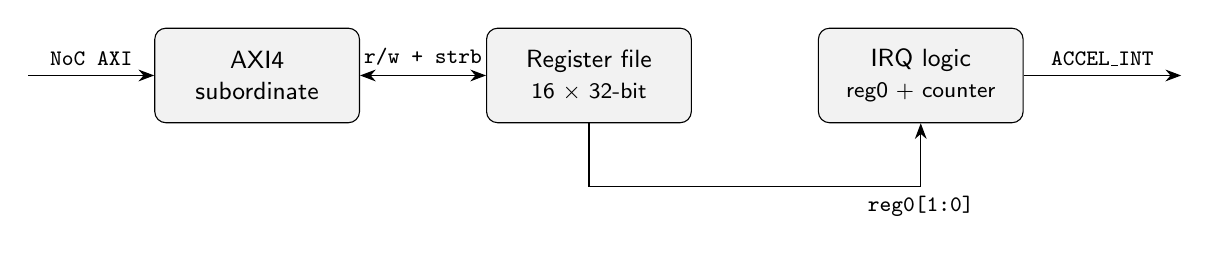
\begin{tikzpicture}[
      font=\small,
      >={Stealth[length=2mm]},
      unit/.style={draw, rounded corners, minimum height=12mm, minimum width=26mm,
                   align=center, fill=black!5},
      lbl/.style={font=\footnotesize\ttfamily},
      node distance=14mm and 16mm
    ]
    \node[unit] (axi)  {AXI4\\ subordinate};
    \node[unit, right=of axi]  (rf)  {Register file\\ \footnotesize 16 $\times$ 32-bit};
    \node[unit, right=of rf]   (ctrl){IRQ logic\\ \footnotesize reg0 + counter};

    \coordinate (axin) at ($(axi.west)+(-16mm,0)$);
    \draw[->] (axin) -- (axi) node[midway,above,lbl]{NoC AXI};
    \draw[<->] (axi.east) -- (rf.west) node[midway,above,lbl]{r/w + strb};
    \draw[->] (rf.south) |- ($(ctrl.south)+(0,-8mm)$) -| (ctrl.south)
              node[pos=0.25,below,lbl]{reg0[1:0]};
    \coordinate (irqout) at ($(ctrl.east)+(20mm,0)$);
    \draw[->] (ctrl.east) -- (irqout) node[midway,above,lbl]{ACCEL\_INT};
  \end{tikzpicture}}
  \caption{High level schematic of the mock accelerator.}
  \label{fig:accel-schematic}
\end{figure}

\section{Register File}
The accelerator holds \texttt{NUM\_REGISTERS} (16 in the base configuration) 32-bit registers. The base
address is defined by the NoC address map (\texttt{0x3000\_0000} in Libre-V); register $i$ is at byte
offset $i \times 4$.

Because the NoC data path is 64 bits wide, the register file is addressed in \emph{even/odd pairs}: one
64-bit beat covers two consecutive 32-bit registers. The hardware forms the pair index from the address
as
\[
  \texttt{idx} = (\texttt{addr[5:2]}) \mathbin{\&} \texttt{4'b1110}
\]
so a beat carries register \texttt{idx} in its low 32 bits and register \texttt{idx+1} in its high 32
bits. A 32-bit access therefore lands in one half of a pair and is steered by the byte strobes: strobes
\texttt{[3:0]} write the even (low) register and strobes \texttt{[7:4]} write the odd (high) register.
Sub-word writes are honoured per byte, so a single-byte store modifies only its byte and leaves the
other three intact.

\begin{docnote}
Register~0 is the control register. When probing the register file with walking patterns, start at
index~1: writing bit~0 of register~0 arms the interrupt (see \autoref{sec:accel-irq}).
\end{docnote}

\section{Register Descriptions}
The registers share one layout: register~0 has the defined control bits below, and registers 1--15 are
plain 32-bit read/write storage.

\regtitle{0}{Accelerator Control Register (CTRL)}

\regmeta{0x3000\_0000}{0x000}{0x00000000}{RW}{Only bits [1:0] are functional; bits [31:2] are storage.}

\begin{register}{H}{Accelerator Control Register (CTRL)}{}

  \regfield[gray!20]{Reserved}{30}{2}{{0}}
  \regfield{IRQ\_CLR}{1}{1}{0}
  \regfield{IRQ\_EN}{1}{0}{0}
  \reglabel{Reset}

  \regfieldvalue[gray!20]{Reserved}{30}{2}{{RW}}
  \regfieldvalue{IRQ\_CLR}{1}{1}{{RW}}
  \regfieldvalue{IRQ\_EN}{1}{0}{{RW}}
  \reglabel{Type}

\end{register}

\textbf{Functional Description.}

Register~0 arms and clears the accelerator interrupt. \textbf{IRQ\_EN} (bit~0) arms the interrupt engine;
\textbf{IRQ\_CLR} (bit~1) acknowledges an asserted interrupt. The upper 30 bits are stored and read back
but have no effect. The behaviour of the interrupt engine is described in \autoref{sec:accel-irq}.

\begin{regmap}
31:2 & reserved & RW & 0 &
Reserved. Stored but have no effect. \\
1    & IRQ\_CLR  & RW & 0 &
Interrupt clear/acknowledge. Writing 1 deasserts an active interrupt and restarts the counter; the bit
self-clears in hardware. \\
0    & IRQ\_EN   & RW & 0 &
Interrupt enable (arm). While 1, the engine counts and asserts the interrupt; while 0, the interrupt is
held deasserted and the counter is reset. \\
\end{regmap}

\regtitle{$i$}{General-Purpose Register (REG$i$), $i = 1 \ldots 15$}

\regmeta{0x3000\_0000}{$i \times$ 0x004}{0x00000000}{RW}{Plain 32-bit storage. Byte-strobe writable.}

\begin{register}{H}{General-Purpose Register (REG$i$)}{}

  \regfield{DATA}{32}{0}{{00000000000000000000000000000000}}
  \reglabel{Reset}

  \regfieldvalue{DATA}{32}{0}{{RW}}
  \reglabel{Type}

\end{register}

\textbf{Functional Description.}

Registers 1 through 15 are general-purpose 32-bit scratch registers with no hardware side effects. In
the mock accelerator they demonstrate the read/write and byte-strobe paths; in a real accelerator they
are where the design places its command, status, and data registers.

\begin{regmap}
31:0 & DATA & RW & 0 &
General-purpose data. Full 32-bit read/write, byte and half-word strobes honoured. \\
\end{regmap}

\section{Interrupt}\label{sec:accel-irq}
The accelerator drives a single interrupt line, delivered to the Rocket's PLIC as source~2
(\texttt{ROCKET\_PLIC\_SRC\_ACCEL}, see \autoref{ch:sw-rocket-sys}). The engine is a simple counter
whose limit is \texttt{ACCEL\_INT\_COUNT} (100 cycles in the base configuration):

\begin{itemize}[nosep]
  \item With \textbf{IRQ\_EN} = 0 the interrupt is held low and the counter is held at 0.
  \item When \textbf{IRQ\_EN} is set to 1 the counter advances each cycle. After
        \texttt{ACCEL\_INT\_COUNT} cycles the interrupt line asserts and \emph{stays} asserted (it is a
        level, not a pulse).
  \item Writing \textbf{IRQ\_CLR} = 1 acknowledges the interrupt: the line deasserts, \textbf{IRQ\_CLR}
        self-clears, and the counter restarts. While the accelerator remains armed it therefore
        re-asserts periodically, once every \texttt{ACCEL\_INT\_COUNT} cycles.
\end{itemize}

\begin{docwarning}
Because the interrupt is a level that re-arms while \textbf{IRQ\_EN} stays 1, an in-flight assertion can
re-appear if the device is cleared without first masking it at the PLIC. To disarm cleanly, mask the
source at the PLIC \emph{first}, then clear \textbf{IRQ\_EN} at the device. A handler should acknowledge
with \textbf{IRQ\_CLR} alone (bit~1), not \texttt{IRQ\_EN|IRQ\_CLR}, so it does not re-arm.
\end{docwarning}

\section{Address Map Summary}

\begin{tabular}{@{}lll@{}}
\toprule
\textbf{Offset} & \textbf{Register} & \textbf{Access} \\
\midrule
0x000        & CTRL (register 0: IRQ\_EN, IRQ\_CLR) & RW \\
0x004--0x03C & REG1--REG15 (general purpose)        & RW \\
\bottomrule
\end{tabular}

\section{Source Files}

\begin{tabular}{@{}ll@{}}
\toprule
\textbf{File} & \textbf{Role} \\
\midrule
\texttt{accelerator/src/accelerator.sv} & Mock accelerator: register file, byte strobes, IRQ counter \\
\texttt{top/noc\_accelerator.sv}        & NoC-side wrapper (struct-to-flat AXI4 subordinate) \\
\bottomrule
\end{tabular}

\newpage

\chapter{Libre Software and Control} 

\section{PicoRV32 Interrupt Handler}

The PicoRv32 core has a built-in controller capable of handling 32 sources. The sources should be wired into the \texttt{irq} input port of the core/package. The handler also controles the \texttt{eoi} (end of interrupt) signals, which go high for the handled interrupt when the specific interrupt handler is called. 

IRQs 0-2 are reserved for internal sources. These include: \begin{enumerate}
      \item IRQ 0 - Timer interrupt
      \item IRQ 1 - EBREAK/ECALL or Illegal INstructions
      \item IRQ 2 - Bus error due to unaligned memory access.  
\end{enumerate}

4 additionals 32-bit regsiters (\texttt{q0-3}) are provided for IRQ handling. WHen the IRQ handler is called, the register \texttt{q0} contains the return address and \texttt{q1} contains the bitmask of all IRQs to be handled. This means one call to the interrupt handler needs to service more than one IRQ when more than one bit is set in \texttt{q1}. When compressed instruction mode is enabled, then the LSB of \texttt{q0} is set when the interrupt instruction is a compressed instruction. This can be userd if the IRQ handler wants to decode the interrupted instruciton. The other additional reisters are uninitializaed and scratch registers. 

Custom instructions defined for interrupt handling: \begin{enumerate}
      \item \texttt{get rd, qs}
      
      Copy the contents from a q-register to a general-purpose register. 
      \item \texttt{retirq}
      
      Return from interrrupt. As side effects, the contents of \texttt{q0} are copied to the program counter and interrupts are re-enabled.
      \item \texttt{maskirq}: 
      
      There is an IRQ MAsk register  containing a birmask of masked interrupts. This instruction writes a new valie to the ieq mask register and reads the old value. 

      \item \texttt{waitirq}
      
      Pause execution until an interrupt becomes pending. 

      \item \texttt{timer}
      
      Reset the timer counter to a new value. The counter counts down clock cycles and triggers the timer interrupt when transitioning from 1 to 0. Setting the counter to zero disables the timer. The old value of the counter is written to rd.
\end{enumerate}

\part{SoC Integration} 
This part is intended for audience intending to understand the platform's architecture and modify/develop their own version at an RTL level. Libre platform is composed of three subsystems:
\begin{itemize}
  \item \hyperref[ch:hw-pico-sys]{Pico Subsystem}
  \item \hyperref[ch:hw-rocket-sys]{Rocket Subsystem}
  \item \hyperref[ch:hw-noc-sys]{Network-on-Chip (NoC) Subsystem}
\end{itemize} 

\chapter{Pico Subsystem}\label{ch:hw-pico-sys}

The Pico subsystem (picosys) is a auxiliary subsystem organized around an AHB-Lite bus. It is used to control the rest of the SoC. The AHB-Lite bus is driven by two managers: COMMCTRL/UART Controller and PicoRV32 core package (picopkg). However, both these managers are time-multiplexed using an AHB MUX, meaning that at any time, there is only a single manager driving the bus. For additional control and interaction, the bus supports a configurable peripheral bus with options like UART, Timers, etc., on-chip SRAM memory, clock and reset generator (CRG), and a bridge to connect to the AXI port of the NoC. 

Picosys uses the CRG to bring up and control the remainder of the SoC. In this chapter, we breakdown the construction and integration of the picosys in Libre-V platform:
\begin{itemize}
  \item \hyperref[sec:hw-picorv32-pkg]{PicoRV32 Core and Package} 
  \item COMMCTRL 
  \item AHB-Lite MUX and Bus
  \item Clock and Reset Generator (CRG)
  \item Peripheral Cluster
  \item On-chip SRAM 
  \item AHB2AXI adapter 
\end{itemize}

\section{PicoRV32 Core and Package}\label{sec:hw-picorv32-pkg}



\newpage



% \chapter{Rocket Subsystem}\label{ch:hw-rocket-sys}

\section{Overview}
This chapter describes how the Rocket core is integrated into Libre-V. The software view --- memory
map, PLIC sources, and the boot handshake --- is in \autoref{ch:sw-rocket-sys}.

The Rocket RTL is not hand-written: it is produced by the \texttt{rocket-chip} generator from a Libre-V
configuration and then wrapped by a single hand-written module that adapts its flat ports to the NoC.

\section{Wrapper}
\texttt{rocket\_subsystem.sv} is the only Rocket RTL authored in this repository. It instantiates the
generated \texttt{ExampleRocketSystem} and:
\begin{itemize}[nosep]
  \item packs the flat \texttt{mem\_axi4} (cacheable) and \texttt{mmio\_axi4} (uncacheable) master ports
        onto the typed FlooNoC request/response structs, exposing them as NoC endpoints
        (\texttt{rocket\_subsystem\_mem} and \texttt{rocket\_subsystem\_mmio}, \autoref{ch:hw-noc});
  \item ties off the debug (DMI/JTAG) interface, which is unused in the base configuration;
  \item takes its clock and active-low reset from the CRG's \texttt{rocket} domain.
\end{itemize}
The split into two master ports is what keeps device registers uncacheable: only \texttt{mem\_axi4}
passes through the coherence hub, while \texttt{mmio\_axi4} bypasses it.

\section{Coherence}
Because this is a bare \texttt{rocket-chip} with no L2, the configuration inserts a \emph{broadcast
coherence hub} (\texttt{TLBroadcast}) between the tile and the memory port
(\texttt{WithCoherentBusTopology}). The hub is not a cache; it serialises and tracks in-flight coherence
transactions so the L1 D-cache stays consistent with external memory. It affects only the cacheable
\texttt{mem\_axi4} path.

\section{Generation Flow}
The committed RTL under \texttt{rocket\_generated/} is a staged copy of the generator's output.

\begin{enumerate}[nosep]
  \item \texttt{LibreRocketConfig.scala} defines the configuration: one big RV64GC core, no virtual
        memory, the two custom AXI master ports, and the coherence topology.
  \item A custom BootROM (\texttt{libre\_bootrom.S}) provides the reset vector, which jumps to DRAM
        (\texttt{0x8000\_0000}) on reset release.
  \item \texttt{generate.sh} builds the BootROM image, elaborates the configuration through mill and
        firtool, and stages the resulting SystemVerilog into \texttt{rocket\_generated/}.
\end{enumerate}

\begin{docnote}
Editing the Rocket therefore means editing \texttt{LibreRocketConfig.scala} (or the BootROM) and
re-running \texttt{generate.sh}; everything downstream (the staged RTL, the wrapper, the SoC build)
follows. The generator tree is used only to \emph{produce} the RTL and is not itself compiled into the
SoC.
\end{docnote}

\section{Source Files}

\begin{tabular}{@{}ll@{}}
\toprule
\textbf{File} & \textbf{Role} \\
\midrule
\texttt{rocket\_subsystem/rocket\_subsystem.sv} & Hand-written wrapper (ports $\to$ NoC structs) \\
\texttt{rocket\_subsystem/rocket\_generated/} & Committed generated RTL \\
\texttt{rocket\_subsystem/generate.sh} & Generation script (BootROM $\to$ elaborate $\to$ stage) \\
\texttt{\ldots/system/LibreRocketConfig.scala} & Rocket configuration \\
\texttt{\ldots/bootrom/libre\_bootrom.S} & Custom reset code \\
\bottomrule
\end{tabular}

\newpage

% \chapter{Network-on-Chip (NoC)}\label{ch:hw-noc}

\section{Overview}
The blocks of Libre-V are tied together by an AXI4 Network-on-Chip generated with
\href{https://github.com/pulp-platform/FlooNoC}{FlooNoC}. Every off-subsystem transfer --- the Pico
reaching a peripheral, the Rocket fetching from its SRAMs, the DMA moving data, an interrupt-driving
device being programmed --- crosses the NoC. It is described declaratively in \texttt{noc\_desc.yml} and
elaborated by \texttt{floogen}; the base configuration uses a single router.

Endpoints are either \emph{managers} (they issue transactions) or \emph{subordinates} (they are
addressed). Managers carry no address range; subordinates own a fixed window in the 32-bit space.

\section{Manager Endpoints}

\begin{tabular}{@{}ll@{}}
\toprule
\textbf{Endpoint} & \textbf{Master} \\
\midrule
\texttt{pico\_subsystem}        & Pico core / COMMCTRL, via the AHB-to-AXI bridge (\autoref{ch:hw-pico-sys}). \\
\texttt{rocket\_subsystem\_mem} & Rocket cacheable port (\texttt{mem\_axi4}). \\
\texttt{rocket\_subsystem\_mmio}& Rocket uncacheable port (\texttt{mmio\_axi4}). \\
\texttt{dma\_mngr}              & DMA datapath (the read/write bursts). \\
\bottomrule
\end{tabular}

\section{Subordinate Endpoints and Address Map}
The subordinate windows below form the system address map for everything reached over the NoC. Local
Pico subordinates (\autoref{ch:sw-pico-sys}) and the Rocket-private devices (\autoref{ch:sw-rocket-sys})
do not appear here --- they never leave their subsystem.

\begin{longtable}{@{}llll@{}}
\toprule
\textbf{Endpoint} & \textbf{Base} & \textbf{Size} & \textbf{Device} \\
\midrule
\endhead
\texttt{uart1}            & \texttt{0x2000\_0000} & 64\,KB  & UART1 (\autoref{ch:sw-uart}) \\
\texttt{timer1}           & \texttt{0x2010\_0000} & 64\,KB  & TIMER1 (\autoref{ch:sw-timer}) \\
\texttt{dma\_sub}         & \texttt{0x2020\_0000} & 64\,KB  & DMA registers (\autoref{ch:sw-dma}) \\
\texttt{accelerator}      & \texttt{0x3000\_0000} & 32\,MB  & Accelerator (\autoref{ch:sw-accel}) \\
\texttt{sram\_imem\_rocket}& \texttt{0x8000\_0000} & 256\,KB & Rocket instruction SRAM \\
\texttt{sram\_dmem\_rocket}& \texttt{0x8010\_0000} & 256\,KB & Rocket data SRAM \\
\texttt{hyperram}         & \texttt{0xA000\_0000} & 256\,MB & External HyperRAM data window \\
\bottomrule
\end{longtable}

\begin{docwarning}
The peripheral band starts at \texttt{0x2000\_0000}, not \texttt{0x1000\_0000}: COMMCTRL intercepts
\texttt{0x1000\_0000} (bus handover) and \texttt{0x1000\_0004} (host interrupt) in its own front-end
before those addresses reach the bus (\autoref{ch:sw-pico-sys}), so \texttt{0x1000\_0000}--\texttt{0x1000\_0FFF}
is reserved and must stay unmapped. Peripherals are spaced 1\,MB apart within the band.
\end{docwarning}

\section{Clock Domains}
Each endpoint belongs to a clock domain, and the top level places an AXI clock-domain-crossing
(\texttt{axi\_cdc}) on the NoC side of each so a block can run at its own frequency. The base
configuration exposes five domains (Pico, Rocket, and one each broadly for the peripheral, HyperRAM, and
accelerator groups), clocked and reset through the CRG (\autoref{ch:sw-crg}).

\begin{docnote}
In the current simulation/testbench setup every domain is driven by the same clock, so the crossings
operate as same-clock passthroughs. The CRG's per-domain clock generation and true frequency ratios are
not exercised in that mode.
\end{docnote}

\section{Top-Level Integration}
\texttt{libre\_top} instantiates the NoC (\texttt{floo\_libre\_v\_noc}) together with every endpoint's
NoC-side wrapper and the clock-domain crossings:

\begin{tabular}{@{}ll@{}}
\toprule
\textbf{Instance} & \textbf{Role} \\
\midrule
\texttt{pico\_subsystem}        & Control plane + Pico manager (\autoref{ch:hw-pico-sys}) \\
\texttt{rocket\_subsystem}      & Rocket manager, cacheable + uncacheable ports (\autoref{ch:hw-rocket-sys}) \\
\texttt{noc\_dma}               & DMA manager + register subordinate \\
\texttt{axi\_mem\_16384x64} ($\times$2) & Rocket instruction/data SRAMs \\
\texttt{noc\_accelerator}       & Accelerator subordinate \\
\texttt{noc\_hyperram}          & HyperRAM controller + data window \\
\texttt{noc\_axi\_uart}         & UART1 subordinate \\
\texttt{noc\_axi\_timer}        & TIMER1 subordinate \\
\texttt{floo\_libre\_v\_noc}    & The generated FlooNoC fabric (router + links) \\
\texttt{axi\_cdc} ($\times$N)   & Per-endpoint clock-domain crossings \\
\bottomrule
\end{tabular}

\section{Source Files}

\begin{tabular}{@{}ll@{}}
\toprule
\textbf{File} & \textbf{Role} \\
\midrule
\texttt{top/libre\_top.sv} & SoC top-level: NoC + all endpoints + clock-domain crossings \\
\texttt{noc/noc\_desc.yml} & Declarative NoC description (endpoints, address map, router) \\
\texttt{noc/hw/} & Generated FlooNoC RTL \\
\bottomrule
\end{tabular}

\newpage


\chapter{On Chip SRAM}

\begin{figure}[htbp]
    \centering
    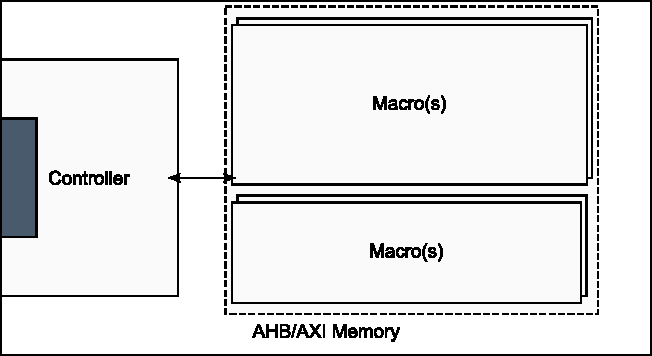
\includegraphics[width=0.55\textwidth]{figures/sram_module_blk.pdf}
    \caption{AXI/AHB SRAM module general block view.}
    \label{fig:sram-module-blk}
\end{figure}

\section{Overview} 
SRAM macros usually expose a simple interface. Such an interface is seldom compatible with the port interfaces exposed by Network on Chip (NoC) or Network Interconnects (NIC). These systems employ elaborate on-chip interconnect standards like AHB/AXI\footnote{None of the AMBA Bus protocols will be discussed in detailed here. Please refer to the \textbf{official} documentation(s) available online.} as they need to handle multiple transactions from multiple devices concurrently. Such protocols include transaction-related metadata signals which enable this capability. We require a controller frontend that will consume these highly informative AHB/AXI transactions and translate it into low-level SRAM interface access(es). We first provide a brief overview of the common controller logic for each of the protocol and then conclude with a description of the generator utility provided. Figure~\ref{fig:sram-module-blk} shows the common block view of the SRAM module. The macros are instantiated independently of the controller via rule checking if using the optional configurator. Named \texttt{gen\_lib\_sram\_*}, the user is expected to replace these prior to synthesis and/or pd with actual models from the foundry.  

\section{AHB Controller}

The AHB family of macros uses \texttt{ahb2sram}, a 32-bit\footnote{At the time of writing this, the controller only supports and is tested for 32-bit word size.} AHB-Lite subordinate for a single-port synchronous SRAM. This controller module is parameterized with the geometry of the module the user expects. This can be different from the configuration of SRAM macros available to the user. The optional generator tool, discussed later, is capable to combining available macros to match the user's specific requirements. 

\underline{Controller Parameters}:
\begin{enumerate}
    \item \texttt{LINE\_W}: required SRAM line width in bits
    \item \texttt{LINE\_AW}: use to define the depth (\(2^{\texttt{LINE\_AW}}\)) of the SRAM in bits
    \item \texttt{WORDS}: number of 32-bit words. The current controller is only capable of supporting 32-bit words. Hence, this parameter should always equal \(\texttt{LINE\_W} / 32\).
\end{enumerate}


\subsection{AHB-Lite Primer}
An AHB-Lite transfer is split across two pipelined phases - address phase (aphase) and data phase (dphase). In the aphase the manager drives \texttt{HADDR}, \texttt{HTRANS}, \texttt{HWRITE}, and \texttt{HSIZE}, qualified by \texttt{HSEL} and the shared \texttt{HREADY}. In the subsequent dphase, write data (\texttt{HWDATA}) or read data (\texttt{HRDATA}) is exchanged, with the subordinate controlling the bus through its registered \texttt{HREADYOUT} and reporting status on \texttt{HRESP}. \texttt{HTRANS[1]} distinguishes an active (\texttt{NONSEQ}/\texttt{SEQ}) beat from \texttt{IDLE}/\texttt{BUSY}. Our implementation does not support burst-type transfers. This is in align with the behavior of the PicoRV32 core's native memory interface. 

\subsection{Phase Sequencing and Timing}
The least significant bits of the address are word alignment bits and will be always zero for word size greater than 8 b. The next significant bit(s) are used for word select for wide SRAM lines.  
An active address beat is registered on \(\texttt{aphase} = \texttt{HSEL}\ \&\ \texttt{HREADY}\ \&\ \texttt{HTRANS[1]}\). A read drives the SRAM in the same cycle and its data is returned in the data phase; a write is held one cycle so that its data phase supplies \texttt{HWDATA}. Consequently a read incurs no wait state and a write incurs exactly one. 

The chip enable, global write enable, and address to the macro are
\[
\texttt{CEN} = \sim(\texttt{read\_en} \mid \texttt{write\_en\_reg}), \quad
\texttt{GWEN} = \texttt{read\_en}, \quad
\texttt{A} = \texttt{read\_en}\ ?\ \texttt{line\_addr\_nxt} : \texttt{line\_addr\_reg},
\]
so a read presents the incoming address immediately while a write replays the registered one.

\subsection{Byte Lanes and Write Enables}
From \texttt{HSIZE} and the lower address bits the controller derives a one-hot-per-byte lane mask (byte, half-word, or full word), registers it into the data phase, and expands it into the macro's active-low, bitwise write enable. When a line is wider and can accomodate several bus-words (\(\texttt{WORDS} > 1\)) the addressed 32-bit word is selected within the line for both the write mask and the read data; otherwise the line is the word. On a read the registered byte lanes gate \texttt{HRDATA}; \texttt{HRESP} is tied to \texttt{OKAY}.

\section{AXI Controller} 

\begin{figure}[htbp]
    \centering
    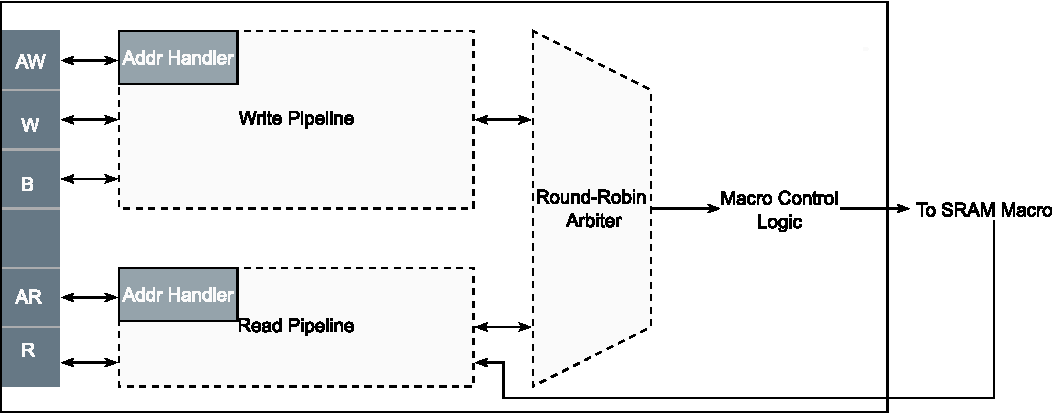
\includegraphics[width=0.75\textwidth]{figures/axi2sram_blk.pdf}
    \caption{\texttt{axi2sram} controller detailed block view.}
    \label{fig:axi2sram-blk}
\end{figure}

Similar to the AHB controller, there is an AXI controller (\texttt{axi2sram}) that converts AXI transactions to SRAM control logic. However, AXI is a more complex (and thereby capable) protocol compared to AHB. Figure~\autoref{fig:axi2sram-blk} provides an overview of the architecture of this controller. Note that the dotted lines are only meant to represent sections of the logic and are not implemented as independent sub-modules. Only the address handler module that is shared by the both pipelines is implemented separately as a module.  

\subsection{AXI Addressing Primer} 

Most of the understanding about AXI addressing has to do with Burst transactions. Burst transactions involve multiple transfers. In these, the manager is expected to provide only a start address and the subordinate is expected to handle the rest of the transfers based on that address and some control signals.  

There are two key control signals:
\begin{enumerate}
    \item \texttt{AxSIZE}: This signal carries information about the number of bytes of information accessed in each transfer (also called a beat) within a Burst transaction. Specifically, 
    \begin{equation*}
        \text{Number of bytes} = 2^{\texttt{AxSIZE}}.
    \end{equation*}
    The width of this signal and the value it can assume is constrained by the data width. AXI doest not permit packet sizes greater than size of the Data bus. The width can be calculated as follows:
    \[
    \text{Width} = \$\texttt{clog2}\left(\frac{\texttt{DW}}{8}\right).
    \]
    (\$\texttt{clog2} rounds up; for a power-of-two \texttt{DW}/8 it is exact.)
    \item \texttt{AxLEN [7:0]}: This indicates the number of transfers to be completed within a single Burst transaction. Specifically,
    \[
    \text{Number of transfers} = 1 + \texttt{AxLEN}
    \] 
\end{enumerate}
Here \texttt{Ax} stands for \texttt{AW} or \texttt{AR}.

There are three types of Burst transactions possible: \begin{itemize}
    \item FIXED: In a Burst type of FIXED type, same address is used repeatedly. An example application provided in the AXI specification is for emptying a FIFO. Generally, used very little.   
    \item INCR: INCR Burst transactions are more common and align with the intuitive picture of a burst transfer. It sequential increments the address until specified.
    \item WRAP: A WRAP Burst transaction is similar to INCR, except it wraps around at a specific boundary depending on transaction attributes. 
\end{itemize}

AXI ``Regular'' transactions impose certain restrictions on the attributes of the trasactions. See section A3.1.8 of AMBA IHI0022 document.  Of those, our address generation submodule (\texttt{axi\_addr\_handler}) assumes the following:
\begin{enumerate}
    \item Number of transfers: INCR bursts of \(1\)--\(256\) beats; WRAP bursts of \(\{2, 4, 8, 16\}\) beats.
    \item Size is the same as the data channnel if Length is greater than 1.
    \item Address is aligned to the transaction container for INCR transactions.
    \item Address is aligned to Size for WRAP transactions.  
    \item Transactions are not permitted to cross a 4KB boundary (section A3.1.3, AMBA IHI0022)
\end{enumerate}

\subsection{Implementation} 

The AXI memory module consists of the following components: Main controller logic for handling AXI transactions, a submodule for handling burst addressing, and the native interfaced, SRAM macro. Here only discuss the controller. The SRAM macro exposes a read port (Q), write port (D), clock (CLK), chip enable port (CEN), global write enable (GWEN), local write enable (WEN), address port (A), and additional signals\footnote{These are ignored for simulation purposes.}, STOV, EMA, EMAS, EMAW.

\begin{enumerate}
    \item Handling the addressing:
    
    The module \texttt{axi\_addr\_handler} is responsible for handling the addressing during Burst transactions. Given a start address, type of burst transfer, size of each transfer, and length of transaction, it generates addresses for each beat of the transaction. It is implemented as a two state FSM: IDLE and ACTIVE. It accepts new start address (called descriptor in the source code) whenever it is in IDLE state. This is indicated to the external environment by asserting the \texttt{start\_addr\_ready} signal. Once the external module asserts \texttt{start\_addr\_valid} signal, this module samples all the input signals, registers them, and enters ACTIVE state. Once in ACTIVE, it uses a count-down timer to track each beat. On the last count, the \texttt{is\_last\_addr} flag is asserted and the FSM moves into IDLE state. The module uses the \texttt{next\_addr\_ready/valid} handshake to move to the next address in the Burst transaction. 

    The next address for Burst transactions is calculated as follows:
    \begin{align}
        \texttt{next\_addr} = \begin{cases}
            \texttt{curr\_addr} & \text{if } \texttt{AxBURST = `FIXED}\\
            \texttt{curr\_addr} + 2^{\texttt{AxSIZE}} & \text{if } \texttt{AxBURST = `INCR} \text{ or within wrap boundary when } \texttt{AxBURST = `WRAP}  \\
            \texttt{wrap\_base} & \text{if } \texttt{AxBURST = `WRAP} \text{ and crossing wrap boundary.}
        \end{cases}
    \end{align}
    Here, \texttt{wrap\_base} is the aligned base of the wrap region. Refer to the AXI specification for how this might be calculated\footnote{WRAP Burst is intended for cache implementations, where, to minimize stall penalty, the first word is delivered immediately and the the rest of the cache line is then fetched sequencially (wrapping).}. This module assumes that the start address is aligned to Size and one increment indicates a word-size (element) increment of \(2^{\texttt{AxSIZE}}\) bytes, i.e., the byte address will be incremented by 4 if Size = 4 bytes. Cache accesses is the main motivation of WRAP Bursts.

    AXI4 limits the length of WRAP transactions to 2/4/8/16. This provides a neat little trick used to calculate the next address in a Wrap transaction without using the modulo operator\footnote{Credits for this trick: \href{https://zipcpu.com/blog/2019/04/27/axi-addr.html}{https://zipcpu.com/blog/2019/04/27/axi-addr.html}.}\footnote{My instinct is that they limit the length for Wrap Bursts for this very reason. Or it may just be that 16 is sufficient for most applications.}. For these Lengths, the value of \texttt{AxLEN} is 0001, 0011, 0111, 1111, respectively. Notice that once the address has been adjusted for word alignment (i.e., those least significant zeros are shifted out), then only the bit positions where there is a 1 in value of \texttt{AxLEN} should be changed in the address (when \texttt{AxLEN}) is aligned with least significant end of the address. Rest of the address should carry over from the before. This trick is realized with the following equation:
    \begin{align}
        \texttt{next\_addr\_wrap} = (\texttt{wrap\_mask}\ \&\ \texttt{next\_addr\_incr}) \mid (\sim \texttt{wrap\_mask}\ \&\ \texttt{curr\_addr}).
    \end{align}
    In the above expression, most of the terms should be self-explanatory, except perhaps \texttt{wrap\_mask}. This term is simply the \texttt{AxLEN} signal shifted to account for the word alignment and padded for address size. Bitwise complement of wrap mask has 1 in bit positions that should not change and be carried over from current address. 

    \item Main Controller Logic 
    
    The main controller is implemented to try and mimic the behavior of \texttt{IntMemAxi} IP from ARM, which is a licensed IP that cannot be open-sourced. However, its functionality is described and can be found \href{https://support.arm.com/documentation/dto0009/a/about-the-internal-memory-interface?lang=en}{here}. However, we cannot guarantee the identical behavior as our development was independent of this IP. 

    This module is designed for controlling a single-port SRAM module. The reads and write paths are implemented independently and arbitrated in a round-robin fashion with reads being the default mode. 
    \underline{Controller Parameters}
    \begin{enumerate}
        \item \texttt{DW}: Word Size (only supports 32/64-bit)
        \item \texttt{IDW}: AXI ID signals width
        \item \texttt{LINE\_W}: required SRAM line width
        \item \texttt{LINE\_AW}: use to define the depth of SRAM (in bits)
        \item \texttt{WORDS}: Number of words per SRAM line 
        \item \texttt{READ\_WAIT}: (0/1) Number of wait stages for reads. 
    \end{enumerate}
    
    This controller can support multiple words per SRAM line. Further, the reads can have an optional wait stage that allows pipelining. Note that like the AHB controller, the WORDS parameter should be sensible and will depend on the word size and the line width.

    The write path is relatively straightforward. Whenever a new write request arrives, the address handler is used to unravel and stream the addresses in the burst sequence. Once available and the previous transaction is completed, a new request write request is raised. 
    
    The read path is slightly more complicated by the optional wait state. Whenever a new read request is granted by the arbiter, the read path becomes busy and the count down timer is topped up. Once the count down is complete, the read value appears on the read port of the macro and is subsequently transferred to \texttt{RDATA} bus when it is available. 

    Both, read and write, paths are pipelined to improve performance. Further, similar to AHB controller, rest of the logic is used to generate the line-wide masks by extending the Strobe signals and word select bits. 
\end{enumerate}

\section{Libremc} 

\begin{docnote}
Terminology: We use ``module'' refers to the entity that actually connects to a bus or a network on chip. The user specifies the module geometry. ``Macro'' is used to refer to the actual SRAM provided by the foundry/memory compilers. Such macros have a primitive interface and might have limited configurations. 
\end{docnote}

We provide a support utility called Libremc (short for Libre macro compiler) that enables the SoC configurator to easily build SRAM modules for connecting to either Pico subsystem or the NoC Subsystem. Consequently, it can configure the \begin{enumerate}
    \item Frontend protocol: Either AXI or AHB.
    \item Width (W): width of the SRAM module.
    \item Depth (D): depth of the SRAM module. 
\end{enumerate}
The word size is fixed to 32 bits for AHB slave memories and to 64 bits for AXI ones\footnote{This is because the bus specifications are a part of the architecture which is common to the platform.}. Further, the address bus width is fixed to 32 bits. 

However, often when synthesizing memory modules, one might not have access to the SRAM compilers or the available compilers might have limited capability and only a few macro configurations are accessible. Libremc allows the user to specify the available macro configurations in a \texttt{.conf} file as follows:

\begin{doccode}
\## Depth        Width   DepthStride  WidthStride  Mask-Granularity
16384          32      0            0            8
16384          64      0            0            8
4096           64      0            0            8
8192           64      0            0            8
512-8192       32      512          0            8
\end{doccode}
The values can be specified explicitly or as (low - high) ranges.  

The tool uses this information to find the ``optimal'' combination to meet the user specified module requirements. To keep things simple, we solve a simple grid problem. For each available macro \(m_i = (w_i, d_i)\) configuration, the following cost function \(f_i\) is evaluated:
\begin{align}
    f_i = c_i \times r_i \times a_i,
\end{align}
where, \(c_i = \mathrm{ceil}(W / w_i)\), \(r_i = \mathrm{ceil}(D / d_i)\), and \(a_i\) is the area of macro. When unavailable, the area of the macro can be estimated as the product of a macro's width \(w_i\) and depth 
\(d_i\)\footnote{This does not capture the wiring overhead and may not correlate well with the actual area. We are working to include this wiring overhead to improve this tool.}. 

The tool selects the configuration as follows:
\begin{enumerate}
    \item Configuration with the lowest value of cost function.
    \item Any ties are broken by choosing the configuration with lowest number of instances (\(r_i \times c_i\)).
    \item Remaining ties are broken by choosing the configuration using the smallest macro.
\end{enumerate}

Once a configuration is found, the tool then automatically generates the module RTL along with a configuration file specifying the chosen macro and grid parameters. In this generated SRAM module it instantiates the requested controller and the grid of macros. In addition, it outputs the word select logic.

\subsection{Usage} 

\begin{enumerate}
    \item Generate a memory module: \begin{verbatim}
        $ make gen PROTO=<ahb|axi> SIZE=<lines>x<width> [MACROLIST=<file>.conf]
    \end{verbatim}
    \item Elaborate and test a generated module: \begin{verbatim}
        $ make test-one PROTO=<ahb|axi> SIZE=<lines>x<width> [EXTRA_AW=n]      
    \end{verbatim} 
    \item Generate and test a memory module in one step: \begin{verbatim}
        $ make test PROTO=<ahb|axi> SIZE=<lines>x<width> [MACROLIST=<file>] [EXTRA_AW=n]
    \end{verbatim}
    \item Clean up generated files: \begin{verbatim}
        $ make clean
    \end{verbatim} 
\end{enumerate}

\section{Summary}

While the AHB controller logic was mostly inherited from Base-SoC (ARM), the AXI controller was developed in-house. AXI's Internal memory interface\footnote{\href{https://support.arm.com/documentation/dto0009/a/about-the-internal-memory-interface?lang=en}{https://support.arm.com/documentation/dto0009/a/about-the-internal-memory-interface?lang=en}} behavior combined with SRAM Macro interface were used as a reference. We improved upon the IntMemAxi module\footnote{We abide by the licensing terms by not using the source code for development of our own version. The functionality has been independently replicated.} by directly supporting AXI4 (it supported AXI3) and directly generating the SRAM interface. 

\begin{docwarning}
Testing the Libremc utility is a non-trivial exercise and in fact a tedious one. Hence, we would appreciate any feedback on the tool, bug finds/fixes in the source code, and inaccuracies in this document.
\end{docwarning}


\end{document}
